% =========================================================================
% REMIX — v3 WORKING DRAFT (full-length; no page budget; trim later)
% Built from the verified v2 tables/proofs with the corrected narrative.
% REMIX — arXiv preprint (Overleaf-compilable, pdfLaTeX)
% Compile: pdflatex main.tex (x2). Figures in figs/*.pdf (upload folder).
% Maps 1:1 onto the AISTATS template for later conversion.
% =========================================================================
\documentclass[twocolumn,10pt]{article}

\usepackage[margin=1in,columnsep=0.25in]{geometry}
\usepackage{amsmath,amssymb,amsthm}
\usepackage{booktabs}
\usepackage{graphicx}
\usepackage{microtype}
\usepackage[numbers,sort&compress]{natbib}
\usepackage{xcolor}
\usepackage[colorlinks=true,linkcolor=blue,citecolor=blue,urlcolor=blue]{hyperref}

\newtheorem{proposition}{Proposition}
\newtheorem{corollary}{Corollary}

\newcommand{\REMIX}{\textsc{Remix}}
\newcommand{\E}{\mathbb{E}}
\newcommand{\Var}{\mathrm{Var}}
\newcommand{\ind}[1]{\mathbf{1}\{#1\}}
\newcommand{\best}[1]{\textbf{#1}}
\newcommand{\secondbest}[1]{\underline{#1}}

\title{Learning to Pool and to Forget:\\
Scalable Empirical-Bayes Forecasting for Intermittent Demand}

\author{Zong-Han Bai \qquad Po-Yen Chu}
\date{}

\begin{document}
\maketitle

\begin{abstract}
Intermittent-demand forecasters routinely fix two structural choices in
advance: \emph{how to pool} evidence across items, and \emph{how to
weight} it over time. We study what happens when both are selected from
data. \REMIX{} is a hierarchical empirical-Bayes forecaster in which an
exponential recency discount is applied to the sufficient statistics used
for both the item-level posterior and the hyperparameter fit, and the
pooling partition (a single pool, the classical taxonomy, or
BIC-selected mixture components) is scored jointly with the discount on
an internal chronological validation split. Estimation stays closed form,
deterministic, and $O(N)$. Classical TSB is a boundary case of the
family, exact under a self-consistent initialization, and a two-sided
credibility bound shows that the discount which keeps the pooled prior
active also shrinks the effective sample behind each group, bounding how
finely a partition can be resolved. Across five public panels (19{,}000+ series) \REMIX{}
attains the best mean scaled pinball loss among non-degenerate methods on
every one, with forgetting responsible for most of the gain. The
advantage widens where it matters most: under strict walk-forward
updating the predictive law beats the best per-block-refit conformal
wrapper by 25\% on mean scaled pinball, and at far-tail quantiles
($q\ge0.95$) the degenerate zero forecast collapses while \REMIX{}
leads.
Finer learned partitions add interpretable structure and cold-start
benefits but little aggregate gain, and simulations with known ground
truth locate the reason: a correct partition does help (on
likelihood-based scores in every cell, on pinball where forgetting is
strong), by more when items hold less of their own history, but the
leverage available here is small. Mean absolute error, the metric
this literature reports most, reverses the sign of that help.
\end{abstract}

% =========================================================================
\section{Introduction}\label{sec:intro}
% =========================================================================

Intermittent demand (long runs of zeros punctuated by sporadic positive
quantities) is pervasive in spare-parts logistics, long-tail e-commerce,
and hospital supply chains. Two modeling traditions address it with
complementary strengths. \emph{Local exponential smoothing} (Croston,
SBA, TSB) \citep{croston1972,syntetos2005accuracy,teunter2011} is
designed to adapt as demand processes drift and die, discounting old
observations at a rate set by a smoothing constant. It is cheap and
reliable, but estimates each series in isolation and does not natively
provide a full predictive distribution. \emph{Hierarchical probabilistic}
approaches \citep{chapados2014,seeger2016,pitkin2024} supply shrinkage
across thousands of sparse series together with calibrated uncertainty.
In their intermittent-demand instantiations they commonly pre-specify the
pooling structure or the temporal evolution, and their inference is
typically heavier than a closed-form update.

Existing procedures therefore tend to fix at least one of two structural
choices: how evidence is shared across items, and how historical
observations are discounted. We represent both choices inside one model
family and select candidate pairs by chronological validation.
Figure~\ref{fig:overview} sketches the resulting design space. The
vertical coordinate is a recency discount $w$ (temporal forgetting). The
horizontal coordinate is the strength of cross-series pooling, which is
not a free parameter we search over but the consequence of two things
we do choose: the partition of items into groups, and the empirical-Bayes
estimate of each group's prior. Classical TSB sits in the no-pooling
region with $w<1$, while stationary hierarchical estimators sit on the $w{=}1$
edge.

The paper's organizing finding is asymmetric, and it is the reason we
report both axes separately. Forgetting is the first-order driver of
forecast improvement. Pooling remains valuable (having \emph{a} shared
prior is worth a great deal), but refining \emph{which} items share it is
often second-order, and we give a reason: forgetting reduces the
effective sample behind each group, and with it the evidence available to
resolve fine structure. Forgetting preserves the need for pooling, but
not necessarily the information needed to estimate a fine pooling
structure.

\begin{figure*}[t]
\centering
\includegraphics[width=0.96\textwidth]{figs/fig1_overview.pdf}
\caption{\textbf{(a)} Two structural axes span classical intermittent-demand
forecasting: cross-series pooling and temporal forgetting $(1-w)$. The
pooling structure and its empirical-Bayes shrinkage jointly determine the
horizontal position: it is not a parameter that is grid-searched
directly. Classical TSB and stationary hierarchical EB each fix one axis.
\REMIX{} selects a candidate configuration on both axes, including the
pooling partition, by chronological validation.
\textbf{(b)} All estimation consumes per-item sufficient statistics, and the
forgetting and pooling candidates are scored jointly, the winning
configuration $(g,w)$ is refit on the full training window, and every
step preserves closed-form, deterministic, $O(N)$ inference.}
\label{fig:overview}
\end{figure*}

Concretely, we build on a hierarchical empirical-Bayes (EB) formulation of
TSB's occurrence--size decomposition (Beta--Binomial occurrence,
log-normal sizes) in which every estimate is a closed-form function of
per-item sufficient statistics. On that representation we make two
compatible modifications. \emph{Recency discounting} replaces each
sufficient statistic by its exponentially weighted analogue, giving every
posterior and every hyperparameter fit a power-prior reading and a
temporal-adaptation capability without changing the asymptotic cost of a
single fit. \emph{Candidate pooling structures} replace the hard-coded
item partition with a small set that includes mixture components learned
by a deterministic EM procedure whose E- and M-steps reuse the model's own
marginals. \REMIX{} scores the resulting candidate configurations
$(g,w)$ on the most recent fraction of the training window and refits the
winner. Total cost is linear in the number of series for a fixed
candidate set.

\paragraph{Contributions.}
\textbf{(1) Method.} A discounted hierarchical empirical-Bayes forecaster
in which the recency discount and the pooling structure are candidate
coordinates rather than fixed choices, selected together by chronological
validation. Inference stays closed form, deterministic, and linear in the
number of series. Neither pooling nor discounting is new on its own. What
we contribute is applying the same recency weighting to the sufficient
statistics used for \emph{both} the item-level posterior update and the
empirical-Bayes hyperparameter fit, and treating the pair $(g,w)$ as
something to select rather than to assume.
\textbf{(2) Theory.} Classical TSB is a boundary case of the family:
Proposition~\ref{prop:tsb-limit} shows the discounted posterior mean
equals the TSB recursion exactly under a self-consistent initialization,
with $O(w^{T})$ discrepancy otherwise. Under forgetting the pooled prior
never loses weight (Proposition~\ref{prop:active}), and finite-sample MSE
bounds under occurrence drift give an $O(\delta^{2/3})$ tracking rate with
$w^{*}\!\to\!1$ as drift vanishes (Proposition~\ref{prop:drift}). Our new
result is the other side of that coin: Proposition~\ref{prop:twosided}
and Corollary~\ref{cor:resolution} give a \emph{practical estimability
condition}: the same reduction in effective sample size that keeps the
prior active also limits how finely a pooling partition can be resolved
from the window by this estimator. Classical credibility
(Proposition~\ref{prop:credibility}) and a finite-class selection
guarantee (Appendix~\ref{app:proofs}) are supporting results, not new.
\textbf{(3) Empirics.} Across five public panels we measure the two axes
separately. Forgetting drives the first-order gains. Differences among
pooling partitions are small on aggregate metrics and survive three
targeted repairs. A controlled study with known ground truth then
separates the explanations: a correct partition improves the
likelihood-based proper scores in every cell and pinball wherever
forgetting is strong (the more so the less history each item has) while
\emph{degrading} mean absolute error, so the flat pooling axis reflects
low leverage on these panels rather than absent structure. That
experiment also gives a controlled instance of a pathology we document on
real data, where a constant-zero forecast attains the lowest MAE on three
of five panels. Probabilistic performance is strong (best mean scaled
pinball among non-degenerate methods on all five panels, a 25\% margin
over the best conformal wrapper under strict walk-forward updating, and
the far-tail lead once the zero forecast's apparent advantage collapses
at $q\ge0.95$), while point performance is competitive but not uniformly
best, including against a tuned-TSB control selected on the same
validation split.

% =========================================================================
\section{Related Work}\label{sec:related}
% =========================================================================

\textbf{Heuristics.} Croston's decomposition \citep{croston1972} smooths
inter-demand intervals and positive sizes. SBA \citep{syntetos2005accuracy}
corrects its bias. TSB \citep{teunter2011} smooths occurrence probability
directly, enabling decay under obsolescence. ADIDA
\citep{nikolopoulos2011} and IMAPA \citep{kourentzes2016} exploit temporal
aggregation. All treat items independently, and their smoothing constants
are the very quantities \REMIX{} learns.

\textbf{Hierarchical and state-space models.} \citet{chapados2014} and
\citet{seeger2016} pool related count series with hierarchical priors at
industrial scale via approximate Bayesian inference. \citet{pitkin2024}
develops hierarchical hurdle models for retail, and iETS
\citep{svetunkov2023iets} gives a likelihood-based state-space treatment.
Many intermittent-demand hierarchical formulations use a pre-specified
temporal evolution or a stationary estimation window, and fix the pooling
structure a priori. Broader dynamic hierarchical models
\citep{westharrison1997} do combine sharing with adaptation, but typically
at the cost of heavier inference than a closed-form update. \REMIX{} keeps
the closed-form EB update and makes both the temporal weighting and the
pooling structure candidate choices.

\textbf{Discounting, power priors, and credibility.} Exponential
discounting of information is a classical device: discount factors are
central to Bayesian dynamic linear models \citep{westharrison1997}, and
raising a likelihood to a power to down-weight historical data is the
power-prior construction of \citet{ibrahimchen2000}. The novelty here is
not the discounting mechanism itself: it is applying the same recency
weighting to the sufficient statistics used for \emph{both} the
item-level posterior update and the empirical-Bayes hyperparameter
estimation (so the group-level priors adapt, and not only the item
states), while everything stays closed form and the discount strength is
selected rather than set. Likewise, the credibility form
$\lambda_i=n_i/(n_i+\phi_g)$ of our posteriors is precisely the actuarial
credibility factor \citep{buhlmann1967}. Proposition~\ref{prop:credibility}
restates that classical theorem in our notation and is not claimed as a
contribution: we invoke it because our new result
(Proposition~\ref{prop:twosided}) concerns when its weight degenerates. On the pooling axis, the local-versus-global tradeoff for
forecasting groups of series is analyzed by
\citet{monteromanso2021}. \REMIX{} treats the pooling \emph{structure}
as one of the candidate choices, and reports what that buys. Count models for intermittent
inventories are developed by \citet{snyder2012}.

\textbf{Evaluation and modern baselines.} High quantiles drive inventory
decisions \citep{kolassa2016}. Pinball is a proper scoring rule
\citep{gneiting2007}, which justifies using it as the selection
criterion. We emphasize scaled pinball loss \citep{makridakis2022} at
$q\ge0.75$ and compare against split-conformal wrappers \citep{lei2018}
(acknowledging that adaptive conformal methods
\citep{gibbs2021} could strengthen these baselines under
nonstationarity), per-series Tweedie regression, the GP--Tweedie suite's
datasets \citep{damato2025}, iETS, and neural models (DeepAR
\citep{salinas2020}, Deep Renewal Processes \citep{turkmen2019}).

% =========================================================================
\section{Method}\label{sec:method}
% =========================================================================

\subsection{Base model: hierarchical EB on sufficient statistics}
\label{sec:base}
Item $i$ has demand $y_{i,t}\ge0$, $t=1,\dots,T_i$. Write
$p_{i,t}=\ind{y_{i,t}>0}$ and $\ell_{i,t}=\log y_{i,t}$ when positive.
Each item belongs to a pooling group $g(i)$ and
\begin{align}
\pi_i &\sim \mathrm{Beta}(\alpha_g,\beta_g), &
p_{i,t}\mid\pi_i &\sim \mathrm{Bern}(\pi_i),\nonumber\\
\mu_i &\sim \mathcal{N}(\mu_{0,g},\tau^2_g), &
\ell_{i,t}\mid\mu_i &\sim \mathcal{N}(\mu_i,\sigma^2_g),
\label{eq:model}
\end{align}
with $y_{i,t}=e^{\ell_{i,t}}p_{i,t}$. Group hyperparameters are fit by
empirical Bayes (Beta--Binomial marginal likelihood; intercept-only REML
for sizes; conjugate scaled-inv-$\chi^2$ item variances), item posteriors
are conjugate, and the point forecast keeps TSB's multiplicative form
$\hat y_i=\hat\pi_i\exp(\hat\mu_i+\tfrac12\hat\sigma^2_i)$. The predictive
law is zero-inflated log-normal
(Appendix~\ref{app:implementation}). Every quantity above is a
function of four per-item sufficient statistics:
$n_i$ (observations), $s_i$ (occurrences), and the sum and sum-of-squares
of positive log-sizes.

\subsection{The forgetting operator}\label{sec:discount}
For $w\in(0,1]$ replace each statistic by its discounted analogue,
\begin{equation}
n_i(w)=\!\sum_{t\le T_i}\! w^{T_i-t},\qquad
s_i(w)=\!\sum_{t\le T_i}\! w^{T_i-t} p_{i,t},
\label{eq:discounted-stats}
\end{equation}
and likewise for the log-size sums. All EB objectives extend to
real-valued pseudo-counts through their log-Gamma representations, so the
\emph{entire} pipeline (hyperparameter fitting included) becomes a
weighted-likelihood (power-prior) scheme, and $w{=}1$ reproduces the
stationary model exactly. The occurrence posterior mean becomes
\begin{equation}
\hat\pi_i(w)
=\lambda_i(w)\,\bar p_i(w)+\bigl(1-\lambda_i(w)\bigr)\mu_{\pi,g},
\label{eq:disc-post}
\end{equation}
with $\bar p_i(w)=s_i(w)/n_i(w)$ and credibility
$\lambda_i(w)=n_i(w)/(n_i(w)+\phi_g)$, $\phi_g=\alpha_g+\beta_g$.

\subsection{The pooling operator}\label{sec:mixture}
Rather than hard-coding $g(\cdot)$, we form candidate partitions:
the single global pool; the classical ADI/CV$^2$ taxonomy
\citep{syntetos2005categorization}; and \emph{learned} partitions in which
the group label is latent and each of $K$ components carries its own
$(\alpha_k,\beta_k,\mu_{0,k},\tau^2_k,\sigma^2_k)$. The item-level
mixture marginal multiplies the Beta--Binomial occurrence evidence by the
Normal random-effects size evidence, so the E-step is closed form and the
M-step maximizes responsibility-weighted versions of the base EB
objectives. Initialization is a deterministic quantile split (the
pipeline stays seed-free) and $K$ is chosen by BIC \citep{keribin2000}.

\subsection{\REMIX{}: joint selection}\label{sec:select}
The last $20\%$ of each training series is held out as an internal
validation block. For every candidate partition and every $w$ on the grid
$\{1,0.999,0.997,0.995,0.99,0.98,0.95,0.90\}$, the model is fit on the
remaining $80\%$ and scored on the block by per-series-scaled pinball loss
over $q\in\{0.5,0.75,0.9\}$. The winning pair $(g,w)$ is refit on the full
window. No out-of-sample data is touched. The selector's cost is a few
dozen closed-form fits: seconds for thousands of series.

\subsection{Theory}\label{sec:theory}
Five results organize this section, in an arc that mirrors the paper's
empirical finding. The first three concern the forgetting axis: classical
TSB is a boundary case of the family
(Proposition~\ref{prop:tsb-limit}), once forgetting is on the pooled
prior never loses relevance (Proposition~\ref{prop:active}), and the
discount trades tracking bias against variance at an explicit rate
(Proposition~\ref{prop:drift}). The remaining two concern what the
selector can and cannot learn: a finite-class selection guarantee
(Proposition~\ref{prop:oracle}, supporting), and a two-sided credibility
bound (the part we consider new) whose corollary limits how finely a
pooling partition can be resolved from a discounted window
(Proposition~\ref{prop:twosided}). After each result we state what it
does and does not establish, and which experiment tests it. Proofs are in
Appendix~\ref{app:proofs}. All statements are also verified
symbolically or numerically in the released test suite. Fix an item.
Let $\hat p_T$ be classical TSB's occurrence
estimate with smoothing $\alpha_p=1-w$ and initialization $\hat p_0$.

\begin{proposition}[TSB is a corner of the plane]
\label{prop:tsb-limit}
For $w\in(0,1)$:
(i) $\lim_{(\alpha,\beta)\to(0,0)}\hat\pi(w)=\bar p(w)$;
(ii) $\hat p_T=(1-w)\sum_{t=1}^{T}w^{T-t}p_t+w^T\hat p_0$ and
$\bar p(w)=(\hat p_T-w^T\hat p_0)/(1-w^T)$;
(iii) hence $\bar p(w)=\hat p_T$ exactly under the self-consistent
initialization $\hat p_0=\bar p(w)$, and $|\bar p(w)-\hat p_T|\le w^{T}$
in general.
\end{proposition}

\emph{What it says, and does not.} Whatever the fifty-year-old
recursion earns on a panel is available to this family by sitting in its
noninformative corner. ``Exact'' holds under the self-consistent
initialization, with $O(w^{T})$ discrepancy otherwise. It does not say
TSB is optimal anywhere. \emph{Tested by:} the corner configuration
reproducing TSB's forecasts numerically, and the identities verified
symbolically in the released test suite.

\begin{proposition}[Forgetting keeps pooling relevant]
\label{prop:active}
For every horizon $T$: $\lambda(w)\le(1+(1-w)\phi)^{-1}<1$ when $w<1$,
whereas $\lambda(1)\to1$ as $T\to\infty$. Under forgetting, the pooled
prior retains strictly positive weight forever: pooling and forgetting
are complements, not substitutes.
\end{proposition}

\emph{What it says, and does not.} Under forgetting, pooling and
forgetting are complements: the shared prior keeps strictly positive
weight at every horizon. It does not say the prior \emph{helps} (that is
Proposition~\ref{prop:credibility}), nor that the item's own data keeps
positive weight (that converse can fail, and
Proposition~\ref{prop:twosided} quantifies exactly when). \emph{Tested
by:} the forgetting rows of the ablation
(Table~\ref{tab:ablation}), where discounting sharpens intervals by
$12\%$ at closer-to-nominal coverage precisely because the prior stays
in force.

\begin{proposition}[Tracking risk under drift]
\label{prop:drift}
If $p_t\sim\mathrm{Bern}(\pi_t)$ independently with
$|\pi_t-\pi_T|\le\delta(T-t)$, then
$|\E\bar p(w)-\pi_T|\le\delta\,w/[(1-w)(1-w^T)]$ and
$\Var\,\bar p(w)\le\tfrac14(1-w)(1+w^T)/[(1+w)(1-w^T)]$, with the
corresponding decomposition for the posterior mean.
\end{proposition}

\begin{corollary}\label{cor:rate}
Balancing the bounds gives $1-w^{*}\asymp\delta^{2/3}$ (with the exact
constant computed in the proof), worst-case MSE $O(\delta^{2/3})$, and
$w^{*}\to1$ as $\delta\to0$: the stationary model is recovered exactly
when nothing drifts, which is the license for selecting $w$ by
validation rather than fixing it.
\end{corollary}

\emph{What it says, and does not.} The optimal discount balances
tracking bias against variance at rate $O(\delta^{2/3})$, recovering the
stationary model exactly as drift vanishes: the license for selecting
$w$ by validation. It does not say the validation-selected $w$ attains
the bound. \emph{Tested by:} the selected discounts tracking apparent
drift across panels (near-stationary RAF selects $w{=}0.997$, drifting
Carparts and M5 select $w{=}0.90$, Figure~\ref{fig:curves}).

\begin{figure}[t]
\centering
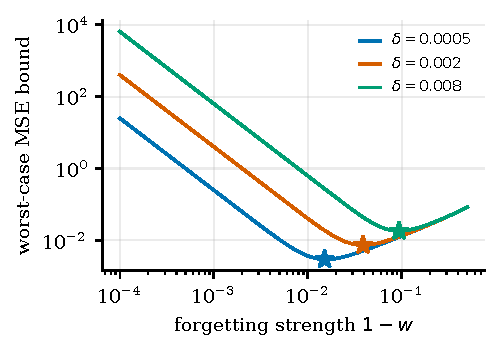
\includegraphics[width=0.93\linewidth]{figs/drift_tradeoff.pdf}
\caption{Proposition~\ref{prop:drift}'s bias--variance bounds. Stars mark
the minimizing forgetting strength; as drift $\delta$ grows the optimum
moves right at the $\delta^{2/3}$ rate of Corollary~\ref{cor:rate}.}
\label{fig:tradeoff}
\end{figure}

\begin{figure}[t]
\centering
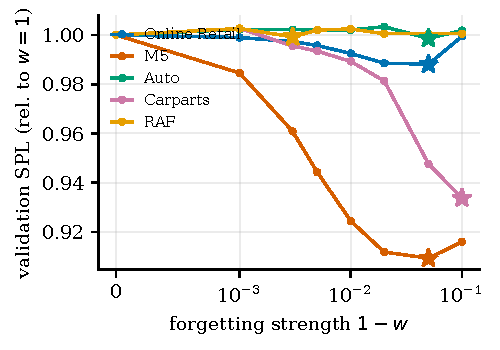
\includegraphics[width=0.93\linewidth]{figs/discount_curves.pdf}
\caption{Validation scaled pinball vs.\ forgetting strength on all five
panels (relative to $w{=}1$; stars = selected $w$). Every curve has an
interior optimum, and its location tracks the panel's apparent
nonstationarity: near-stationary RAF selects $w{=}0.997$, drifting
Carparts selects $w{=}0.90$, matching Figure~\ref{fig:tradeoff}.}
\label{fig:curves}
\end{figure}

Figure~\ref{fig:curves} shows the theory operating in practice: each
dataset's validation curve is convex with an interior minimum whose
location orders the panels by nonstationarity.

Finally, the selection step itself admits a guarantee. The selector
compares a \emph{finite} set of $M$ candidate configurations (here
$M=24$: eight discounts $\times$ three partitions) by their average
scaled pinball loss on $n$ held-out validation observations.

\begin{proposition}[Oracle inequality for the selector]
\label{prop:oracle}
Let $R(c)$ denote the expected validation risk of candidate $c$ and
$\hat R(c)$ its empirical average over the $n$ validation observations.
Assume the per-observation scaled pinball scores lie in $[0,B]$ and are
independent across items conditional on the fitted candidates. Then the
selected $\hat c=\arg\min_c \hat R(c)$ satisfies, with probability at
least $1-\eta$,
\[
R(\hat c)\;\le\;\min_{c} R(c)\;+\;B\sqrt{\frac{2\log(2M/\eta)}{n}} .
\]
\end{proposition}

This is the standard finite-class uniform-convergence argument
(Appendix~\ref{app:proofs}), and we report it as a supporting result
rather than a contribution. Two caveats govern how much it delivers.
First, the independent units are \emph{items}, not observations:
within-series temporal dependence makes an item's validation scores
correlated, so we aggregate each item's validation loss into one number
and take $n$ to be the number of validation items ($n=3649$ on Online
Retail), not the ${\sim}8\times10^4$ observation-quantile pairs. Second,
boundedness is not automatic (the per-series scaling divides by mean
absolute demand), so $B$ must be read as a clipping level applied to the
per-item loss. With $M=24$, $\eta=0.05$ and $n=3649$ the penalty is
$0.061\,B$. Since the observed spread of mean SPL across pooling
structures is about $0.004$, the bound is nowhere near tight enough to
certify one partition over another. We take that as corroboration rather
than as a defect: it is the same conclusion the ablation reaches
empirically in Section~\ref{sec:ablation}, namely that partition-level
differences on these panels are not statistically resolvable, while the
bound does still rule out the selector settling on a badly worse corner.

\begin{proposition}[Pooling reduces risk; classical credibility]
\label{prop:credibility}
Under model \eqref{eq:model} with known hyperparameters, the posterior
mean \eqref{eq:disc-post} is the Bayes estimator of $\pi_i$ under
squared loss, and its Bayes risk is strictly smaller than that of the
per-item empirical rate $\bar p_i$ whenever $\phi_g>0$. The optimal
weight is exactly the credibility factor
$\lambda_i=n_i/(n_i+\phi_g)$ of \citet{buhlmann1967}. (Statement and
classical proof in Appendix~\ref{app:proofs}.)
\end{proposition}

Proposition~\ref{prop:credibility} is not new: it is the
B\"uhlmann--Straub credibility theorem specialized to Bernoulli
occurrences. Stating it makes the division of labor exact: pooling
carries the cross-sectional risk reduction
(Proposition~\ref{prop:credibility}), forgetting carries the temporal
adaptation (Propositions~\ref{prop:tsb-limit}--\ref{prop:drift}), and
validation carries the choice between them
(Proposition~\ref{prop:oracle}). The division is tested directly by the
simulation of Section~\ref{sec:synthetic}: its no-pooling arm loses to a
single pooled prior in every cell, by more the more heterogeneous the
panel, with Proposition~\ref{prop:credibility} operating as stated.

\subsection{How much structure is estimable?}\label{sec:resolution}

Propositions~\ref{prop:active} and \ref{prop:credibility} both argue in
one direction: the pooled prior never becomes irrelevant. The converse
direction turns out to govern what a \emph{learned} partition can
deliver, and it is the reason the pooling axis behaves the way
Section~\ref{sec:ablation} reports. Write the size block of
\eqref{eq:model} in credibility form: item $i$ in group $g$ carries
$n_i$ discounted positive observations and shrinkage weight
$\lambda_i=n_i/(n_i+\kappa_g)$ with $\kappa_g=\sigma_g^2/\tau_g^2$,
while the group variance component is estimated by the
moment/REML solution $\hat\tau_g^2=\max(0,\,S_g^2-\bar s_g)$, where
$S_g^2$ is the empirical variance of the $m_g$ item means in $g$, and
$\bar s_g=m_g^{-1}\sum_{i\in g}\sigma_g^2/n_i$ is their average
sampling variance.

\begin{proposition}[Two-sided credibility; the collapse event]
\label{prop:twosided}
\textbf{(i)} For $w<1$,
$\lambda_i\le\bigl[1+(1-w)\kappa_g\bigr]^{-1}<1$.
\textbf{(ii)} With $S_g^2$ the unweighted sample variance of the item
means normalized by $1/(m_g-1)$, and $\bar s_g$ the unweighted mean of the
$s_i$, $\mathbb{E}[S_g^2]=\tau_g^2+\bar s_g$ holds \emph{exactly} for
independent items with heteroskedastic $s_i$: no balance assumption and
no weighting correction is needed. Under the Gaussian working model
\[
\Pr\bigl[\hat\tau_g^2=0\bigr]\;\simeq\;
\Phi\!\Bigl(-\sqrt{\tfrac{m_g-1}{2}}\,\rho_g\Bigr),
\qquad
\rho_g:=\frac{\tau_g^2}{\tau_g^2+\bar s_g}\in(0,1).
\]
Since $n_i\le(1-w)^{-1}$ we have $\bar s_g\ge(1-w)\sigma_g^2$ and hence
$\rho_g\le\tau_g^2/[\tau_g^2+(1-w)\sigma_g^2]$: \emph{forgetting lowers
the resolution ratio}. On the event $\hat\tau_g^2=0$ the plug-in weight is
$\lambda_i=0$ and the item's own history is discarded entirely.
The population ratio $\rho_g$ is not observable. Its signed sample
analogue, which is what we report, is
$\hat z_g=(S_g^2-\bar s_g)/\widehat{\mathrm{SE}}(S_g^2)$ with
$\widehat{\mathrm{SE}}(S_g^2)=\sqrt{2/(m_g-1)}\,S_g^2$, so that
$\hat z_g\le0$ is exactly the collapse event. We keep the two symbols
distinct throughout: $\rho_g\in(0,1)$ is a population quantity,
$\hat z_g\in(-\infty,\sqrt{(m_g-1)/2}\,]$ is a statistic.
\textbf{(iii)} If the variance components are partially pooled,
$\tilde\tau_g^2=\omega_g\hat\tau_g^2+(1-\omega_g)\hat\tau_0^2$ with
$\omega_g<1$ and $\hat\tau_0^2>0$, then
\[
\lambda_i\;\ge\;
\frac{n_i(1-\omega_g)\hat\tau_0^2}
     {n_i(1-\omega_g)\hat\tau_0^2+\sigma_g^2}\;>\;0 .
\]
\end{proposition}

\begin{corollary}[Variance-component resolution condition]
\label{cor:resolution}
Under this estimator and window, a group's variance component is
reliably estimable only where $\rho_g\sqrt{m_g-1}\gtrsim1$, equivalently
$\tau_g^2\gtrsim\bar s_g/(\sqrt{m_g-1}-1)$ with
$\bar s_g\ge(1-w)\sigma_g^2$. Refining a partition lowers $\tau_g^2$
(members are alike by construction) and $m_g$ (fewer members per group),
while forgetting raises the floor on $\bar s_g$. All three move the group
toward the collapse event. Past that point the regularized estimate
returns $\tilde\tau_g^2\to\hat\tau_0^2$, so an over-fine partition
degrades to the \emph{global pool} rather than to group means.
\end{corollary}

\emph{What this says and does not say.} It is an estimator- and
window-specific statement about \emph{estimability}: with these
sufficient statistics, this moment/REML estimator, and this much
discounted data, finer structure cannot be resolved reliably. It is
\emph{not} an information-theoretic impossibility result (we prove no
lower bound over all estimators), and it says nothing about which
partition is best \emph{below} the threshold. Section~\ref{sec:synthetic}
tests it directly on data with known ground truth, where the true
partition is available as a control.

Parts (i) and (iii) together place $\lambda_i$ strictly inside $(0,1)$:
under forgetting plus partial pooling of the variance components,
neither the shared prior nor the item's own history can be washed out.
Without (iii) only the upper bound survives, and the lower one fails
exactly on the event quantified in (ii). Three consequences organize the
rest of the paper. First, the collapse is \emph{driven by the
interaction} of the two axes rather than by either alone: forgetting
supplies the small effective sample, a learned partition supplies the
small within-group spread. Second,
Corollary~\ref{cor:resolution} predicts a ceiling on partition refinement
for the present estimator: the available window cannot reliably support
finer structure, whatever tuning is applied to this estimator. Third, it explains why the risk surface over
partitions is flat near its optimum: candidates beyond the resolution
limit are automatically neutralized toward the global pool, so
Proposition~\ref{prop:oracle}'s selector is choosing among configurations
that the data cannot distinguish. Section~\ref{sec:ablation} measures all
three. Proofs are in Appendix~\ref{app:proofs}. Every step of
Propositions~\ref{prop:tsb-limit}--\ref{prop:drift} and
\ref{prop:twosided} is verified symbolically in the released test suite,
with the one approximation in (ii) checked against simulation.

\subsection{Computational profile}\label{sec:complexity}
One pass computes all statistics in $O(\sum_i T_i)$; each EB fit is a
two-parameter optimization per group; mixture EM adds $O(NK)$ per
iteration; selection multiplies a constant number of fits; prediction is
$O(N)$ (point) or $O(NQ)$ (quantiles). Everything is
deterministic: repeated runs are bit-identical, which we verify with an
automated test in the released code.

% =========================================================================
\section{Experiments}\label{sec:experiments}
% =========================================================================

\subsection{Setup}\label{sec:setup}
\textbf{Datasets.} Two daily panels: \textbf{Online Retail} \citep{chen2015}
(3{,}649 series; first third initializes, rest evaluates) and a
seed-controlled 5{,}000-series \textbf{M5} sample \citep{makridakis2022}
(init ratio $2/3$, which keeps the slower baselines affordable; a
full-scale 30{,}490-series run against the fast classical methods
confirms it is representative, with \REMIX{} best on all three point
metrics at full scale, Appendix~\ref{app:extra}), plus the monthly
intermittent suite of
\citet{damato2025} with their exact last-$h$ holdout: \textbf{Auto}
(3{,}000 series, $T{=}18$, $h{=}6$), \textbf{Carparts} (2{,}509, $T{=}45$,
$h{=}6$), \textbf{RAF} (5{,}000, $T{=}72$, $h{=}12$).
\textbf{Baselines.} Croston, SBA, TSB, ADIDA, IMAPA, AutoARIMA, AutoTheta
(StatsForecast); a tuned-TSB control (\emph{TSB-tuned}: 25-candidate
$(\alpha_d,\alpha_p)$ grid scored on the same internal chronological
split \REMIX{} selects on, Appendix~\ref{app:implementation}); per-series autoregressive Tweedie GLM (\emph{not} the GP-based method of \citealt{damato2025}); split-conformal
wrappers (CP-$\ast$) of the point methods for probabilistic comparison;
iETS \citep{svetunkov2023iets}; neural comparisons in
Appendix~\ref{app:extra}.
\textbf{Protocols.} The fixed-origin protocol fits once on the
initialization window and scores the full evaluation span. On Online
Retail this spans several months, matching review cycles in slow-moving
spare-parts management where a demand-rate estimate is fixed between
periodic replenishment reviews. Because such a protocol structurally
favors stable intensity estimation, we complement it in two ways:
Figure~\ref{fig:horizon} decomposes error by forecast horizon, showing
the advantage is not an artifact of averaging over long horizons, and
Section~\ref{sec:walkforward} evaluates all methods under strict
block-wise walk-forward updating.

\begin{figure}[t]
\centering
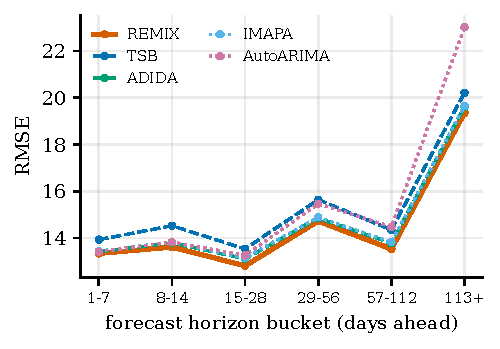
\includegraphics[width=0.93\linewidth]{figs/horizon_decomp.pdf}
\caption{Online Retail: RMSE by forecast-horizon bucket. \REMIX{} has
the lowest RMSE in \emph{every} bucket, from days 1--7 onward; its edge
is not produced by long-horizon averaging. (On MAE the per-bucket
differences among the leading methods are within 1--2\%.)}
\label{fig:horizon}
\end{figure}

\textbf{Metrics.} Point: MAE and RMSSE (per-series scaled). Probabilistic:
scaled pinball loss (SPL, M5-Uncertainty scaling) with emphasis on
$q\ge0.75$, plus Coverage@80/AIW@80. All quantiles of all methods are
zero-truncated and monotonized. \REMIX{} is reported \emph{raw} (the
optional calibration layer is off unless stated). Paired per-series
significance tests are Holm-adjusted.

\subsection{Main results}\label{sec:main-results}

\begin{table*}[t]
\centering
\caption{\textbf{Point forecasting} across the five panels: MAE and RMSSE
(lower is better; bold best, underline second, computed over the
non-degenerate methods). The deliberately included degenerate rows (Zero,
Naive-last) are excluded from ranking: the Zero forecast attains the
lowest MAE on three panels, which is a known pathology of MAE on
intermittent data and the reason RMSSE and probabilistic metrics carry
the evaluation (see text). \REMIX{} is one model with its pooling
structure and discount selected on the internal validation
split: selected configuration shown beneath the table.}
\label{tab:point}
\small
\setlength{\tabcolsep}{3.4pt}
\begin{tabular}{lcc@{\hspace{10pt}}cc@{\hspace{10pt}}cc@{\hspace{10pt}}cc@{\hspace{10pt}}cc}
\toprule
 & \multicolumn{2}{c}{Online Retail} & \multicolumn{2}{c}{M5} & \multicolumn{2}{c}{Auto} & \multicolumn{2}{c}{Carparts} & \multicolumn{2}{c}{RAF}\\
\cmidrule(lr){2-3}\cmidrule(lr){4-5}\cmidrule(lr){6-7}\cmidrule(lr){8-9}\cmidrule(lr){10-11}
Model & MAE & RMSSE & MAE & RMSSE & MAE & RMSSE & MAE & RMSSE & MAE & RMSSE\\
\midrule
CrostonClassic & 6.3294 & 5.1051 & 1.2345 & 2.3539 & 3.4056 & 1.1488 & 0.6792 & 1.0981 & 2.7315 & 1.6280\\
CrostonSBA & 6.1953 & 5.0692 & 1.2076 & 2.3517 & \secondbest{3.3325} & \best{1.1451} & 0.6628 & 1.0935 & 2.6520 & 1.6272\\
TSB & \best{5.5736} & 4.8031 & 1.2672 & 2.3612 & 3.6587 & 1.2066 & \best{0.5396} & 1.0156 & \best{2.1660} & 1.6570\\
TSB-tuned & \secondbest{5.6318} & 4.7985 & \secondbest{1.1932} & \secondbest{2.3137} & 3.3917 & \secondbest{1.1452} & \best{0.5396} & 1.0156 & \secondbest{2.2447} & 1.6408\\
ADIDA & 5.6860 & \secondbest{4.7967} & 1.2274 & 2.3398 & 3.4079 & 1.1545 & 0.5556 & 1.0244 & 2.2977 & \best{1.6245}\\
IMAPA & 5.7000 & 4.7970 & 1.2317 & 2.3280 & 3.4143 & 1.1555 & \secondbest{0.5524} & 1.0126 & 2.2850 & 1.6259\\
AutoARIMA & 6.5494 & 4.8175 & 1.2283 & 2.3169 & 3.4417 & 1.1745 & 0.5822 & \secondbest{1.0105} & 2.3153 & 1.6262\\
AutoTheta & 8.2862 & 4.8550 & 1.2988 & 2.3143 & 3.7490 & 1.2215 & 0.5704 & \best{0.9966} & 2.3687 & 1.6399\\
\midrule
Zero & 4.7549 & 4.8089 & 1.2995 & 2.4629 & 4.1444 & 1.4454 & 0.3867 & 1.0949 & 1.1717 & 1.6345\\
Naive-last & 6.0570 & 4.8324 & 1.3750 & 2.5450 & 4.3529 & 1.3818 & 0.5399 & 1.1408 & 1.8340 & 1.7644\\
\midrule
\REMIX{} (ours) & 5.6639 & \best{4.7879} & \best{1.1774} & \best{2.2724} & \best{3.3269} & 1.1455 & 0.5714 & 1.0286 & 2.3233 & \secondbest{1.6256}\\
\bottomrule
\end{tabular}

\smallskip
{\footnotesize Selected $(g,w)$ per dataset: Online Retail:
(mixture, $0.98$); M5: (mixture, $0.90$); Auto: (mixture, $0.995$);
Carparts: (mixture, $0.90$); RAF: (mixture, $0.997$). The selector chose
the learned partition on every panel.}
\end{table*}

\begin{table*}[t]
\centering
\caption{\textbf{Probabilistic forecasting}: scaled pinball loss, mean
over $q\in\{0.1,0.25,0.5,0.75,0.9\}$ and at the inventory-critical q90.
\REMIX{} predictive distributions are raw (no post-hoc calibration);
marks rank the non-degenerate methods.
$^{\dagger}$On RAF the degenerate all-zero forecast attains marginally
lower SPL than every method: evidence that $q\le0.9$ evaluation
saturates on this ultra-sparse panel (see text).}
\label{tab:prob}
\small
\setlength{\tabcolsep}{3.2pt}
\begin{tabular}{lcc@{\hspace{9pt}}cc@{\hspace{9pt}}cc@{\hspace{9pt}}cc@{\hspace{9pt}}cc}
\toprule
 & \multicolumn{2}{c}{Online Retail} & \multicolumn{2}{c}{M5} & \multicolumn{2}{c}{Auto} & \multicolumn{2}{c}{Carparts} & \multicolumn{2}{c}{RAF}\\
\cmidrule(lr){2-3}\cmidrule(lr){4-5}\cmidrule(lr){6-7}\cmidrule(lr){8-9}\cmidrule(lr){10-11}
Model & Mean & q90 & Mean & q90 & Mean & q90 & Mean & q90 & Mean & q90\\
\midrule
AutoARIMA & \secondbest{1.0159} & 1.6365 & 2.9721 & 3.1439 & \secondbest{0.3189} & \secondbest{0.2659} & 0.4084 & 0.4897 & 0.4020 & 0.5910\\
AutoTheta & 1.0193 & \secondbest{1.6285} & 2.2205 & 2.7309 & 0.3403 & 0.2760 & 0.3925 & \best{0.4697} & 0.4104 & 0.5956\\
CP-Croston & 1.4595 & 2.6916 & 1.8110 & 2.2595 & 0.3260 & 0.3105 & 0.4012 & 0.5433 & 0.3322 & 0.4927\\
CP-SBA & 1.4618 & 2.7806 & 1.8035 & 2.2589 & 0.3256 & 0.3153 & 0.3982 & 0.5418 & 0.3290 & 0.4920\\
CP-TSB & 1.1709 & 2.6418 & 1.9930 & \best{2.1521} & 0.3459 & 0.3150 & 0.3783 & \secondbest{0.4842} & 0.3814 & 0.4986\\
CP-ADIDA & 1.1251 & 2.5118 & 1.8011 & 2.2626 & 0.3275 & 0.3082 & 0.3571 & 0.4982 & \secondbest{0.3097} & 0.4905\\
CP-IMAPA & 1.1292 & 2.5212 & \secondbest{1.7945} & \secondbest{2.2304} & 0.3279 & 0.3084 & \secondbest{0.3561} & 0.4908 & 0.3116 & 0.4907\\
Tweedie-GLM & 1.1477 & 1.7458 & 3.8859 & 5.0919 & 0.3221 & 0.2783 & 0.4776 & 0.6897 & 0.3121 & 0.5312\\
iETS & 1.0878 & 1.9332 & 2.4291 & 3.4758 & 0.3448 & 0.3252 & 0.4561 & 0.5646 & 0.3494 & \secondbest{0.4900}\\
\midrule
Zero & 0.9224 & 1.6604 & 1.9590 & 3.5262 & 0.5612 & 1.0102 & 0.3736 & 0.6725 & 0.2669$^{\dagger}$ & 0.4805$^{\dagger}$\\
\midrule
\REMIX{} (ours) & \best{0.8843} & \best{1.5262} & \best{1.6992} & 2.4688 & \best{0.2957} & \best{0.2647} & \best{0.3305} & 0.4916 & \best{0.2681} & \best{0.4862}\\
\bottomrule
\end{tabular}
\end{table*}

\begin{figure}[t]
\centering
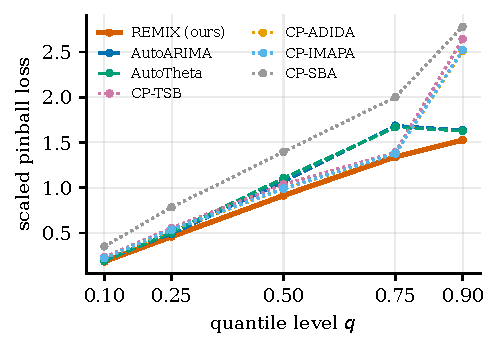
\includegraphics[width=0.93\linewidth]{figs/spl_profile.pdf}
\caption{Scaled pinball by quantile on Online Retail. Conformal wrappers
are competitive at central quantiles but degrade sharply at q90, exactly
where inventory decisions live \citep{kolassa2016}. \REMIX{} dominates the
entire profile.}
\label{fig:profile}
\end{figure}

Tables~\ref{tab:point} and \ref{tab:prob} contain the headline evidence.
\textbf{Point:} \REMIX{} takes the most first places (4 of 10 columns:
both M5 columns, Online Retail RMSSE, Auto MAE) and is in the top two on
5 of 10 (a sixth, Auto RMSSE, trails the runner-up by $0.0003$). TSB
follows with three MAE wins (sharing the Carparts win with its tuned
variant), and no other baseline is best more than once. More telling
than the win count is the consistency: on the columns where \REMIX{} is
outside the top two it sits within 8\% of the leader (within 2\% on
Online Retail MAE and Auto RMSSE), whereas every classical method
has at least one panel where it trails badly (TSB's Auto MAE is 10\%
off; AutoTheta's Online Retail MAE is 49\% off). On the short monthly panels the
differences among leading methods are small, and the decision-relevant
comparison is probabilistic \citep{kolassa2016}.

The TSB-tuned row is the fairness control that
Proposition~\ref{prop:tsb-limit} makes obligatory: if the two knobs are
the same knob, TSB deserves the same selection treatment \REMIX{}
receives. Grid-searching $(\alpha_d,\alpha_p)$ on the identical internal
split under a scaled criterion (Appendix~\ref{app:implementation}) moves
$\alpha_p$ from the textbook $0.45$ to $0.25/0.01/0.10$ on the three
daily-or-large panels, the direction the family view predicts, and
closes much of the point gap on M5 and Auto. It also cuts the other way
twice: on Online Retail and RAF the tuned constants \emph{lose} raw MAE
to the textbook ones, because the scaled criterion steers TSB away from
the zero-leaning configurations that MAE rewards (the pathology
quantified below), and on Carparts the search returns the textbook
constants unchanged. \REMIX{} retains the best RMSSE on Online Retail
and M5 and the probabilistic lead on every panel. \textbf{Probabilistic:} \REMIX{} attains the best mean SPL among
non-degenerate methods on all five panels (by 13\% over the runner-up on
Online Retail, 5\% on M5, and 7--14\% on the monthly suite) and the best
q90 on Online Retail, Auto, and RAF. The qualifier matters on RAF, where
the all-zero forecast attains a marginally lower mean SPL than every
method: at that sparsity the quantile levels we report are largely
saturated. Extending the evaluation to $q\in\{0.95,0.975,0.99\}$
resolves the saturation (Appendix~\ref{app:fartail}): the zero forecast
falls behind every intensity-bearing method from $q{=}0.95$ on, and
\REMIX{} takes the far tail on both sparse panels (best in five of six
cells, near-tied with AutoARIMA in the sixth). Figure~\ref{fig:profile}
shows the mechanism on the retail panel: conformal wrappers are
competitive near the median but degrade sharply at upper quantiles under
the present split-conformal construction, while the zero-inflated
log-normal EB law keeps sharp, calibrated tails (on M5, CP wrappers
remain strong at q90 specifically. \REMIX{}'s lead there is the full
distribution). We test one static split-conformal variant. Adaptive,
rolling, and weighted conformal constructions are designed for exactly
the nonstationarity at issue here and are not evaluated, so this is a
statement about our wrapper, not about conformal prediction. iETS and
Tweedie-GLM trail \REMIX{} at every reported cell. The raw law over-covers
mildly on Online Retail (Coverage@80 $=0.896$, AIW $10.34$,
Table~\ref{tab:coverage}). With the optional calibration layer switched
on \emph{in both configurations being compared}, the forgetting
configuration reaches coverage $0.837$ at AIW $8.96$ versus the
stationary configuration's $0.845$ at $10.03$: $11\%$ narrower
intervals at closer-to-nominal coverage.

\paragraph{Degenerate baselines as measurement instruments.} We include
the all-zero and naive-last forecasts deliberately, because on
intermittent data they calibrate what the metrics can and cannot see.
The Zero forecast attains the lowest MAE on three of five panels (e.g.,
$4.75$ on Online Retail, below every real method): absolute error is
minimized by predicting the conditional median, which on these panels is
zero. The reading we draw is about the metric, not about any method that
scores well on it: MAE on highly intermittent panels rewards
conservative zero-leaning forecasts and should be interpreted jointly
with scaled-error and distributional metrics. This is the
quantitative footnote to every MAE column in Table~\ref{tab:point}
(in particular, TSB's three MAE wins should be read in light of the fact
that an even more zero-leaning forecast wins those columns
outright), and it is why RMSSE and the probabilistic metrics carry our
evaluation \citep{kolassa2016}. The same instrument exposes a limit of
quantile evaluation itself: on RAF, the sparsest panel, the Zero
forecast attains marginally lower mean SPL than every method
($0.2669$ vs.\ \REMIX{}'s $0.2681$), because for most RAF series the
true demand quantiles up to $q{=}0.9$ \emph{are} zero. On such panels
only the far tail ($q>0.9$) and interval-based diagnostics
(Table~\ref{tab:coverage}) discriminate between methods, and running
that far-tail evaluation (Appendix~\ref{app:fartail}) confirms the
reading: the zero forecast drops to last from $q{=}0.95$ on, and
\REMIX{} leads it.

\subsection{What does the selector learn?}\label{sec:selector}

\begin{table}[t]
\centering
\caption{Learned mixture components on Online Retail ($K{=}5$ by BIC),
sorted by occurrence level. $\phi_k=\alpha_k+\beta_k$ is the pooling
strength the component assigns to its members.}
\label{tab:components}
\small
\setlength{\tabcolsep}{4.2pt}
\begin{tabular}{ccccc}
\toprule
Comp. & Weight & Occ.\ prior mean & $\phi_k$ & Median size\\
\midrule
1 & 0.20 & 0.048 & 79.4 & 1.4\\
2 & 0.19 & 0.096 & 27.8 & 5.5\\
3 & 0.10 & 0.155 & 495.9 & 2.5\\
4 & 0.33 & 0.320 & 15.5 & 4.4\\
5 & 0.19 & 0.571 & 12.3 & 12.2\\
\bottomrule
\end{tabular}
\end{table}

Three consistent behaviors emerge across panels. \textbf{(i) The plane is flat near its
optimum, exactly as Proposition~\ref{prop:oracle} predicts.} Re-running
the selector with validation ratios $\{0.1,0.2,0.3\}$ on Online Retail
selects (global, $0.95$), (mixture, $0.98$), and (mixture, $0.95$)
respectively, yet all three land in a tight out-of-sample band (MAE
$5.53$--$5.66$, RMSSE $4.788$--$4.793$), each better than the
stationary corner's MAE $5.766$. With $n=3{,}649$ validation items (the
bound's independent units, Proposition~\ref{prop:oracle}) and $24$
candidates, the oracle bound makes near-optimal
configurations statistically indistinguishable. The selector's job is to
avoid the bad corners, not to locate a knife-edge optimum.
\textbf{(ii) The selected discount tracks apparent drift}
(Figure~\ref{fig:curves}): near-stationary RAF selects $w{=}0.997$ while
drifting Carparts and M5 select $w{=}0.90$, the qualitative signature of
Corollary~\ref{cor:rate}. \textbf{(iii) The selector consistently picks
the learned partition ($K\in\{4,5,6\}$ on all five panels), but
partition-level differences are small on aggregate metrics.} On Online Retail the
ablation of Section~\ref{sec:ablation} shows all three partitions within
$0.7\%$ of one another on every metric, point and probabilistic alike.
The five-panel grid (Appendix~\ref{app:extra}) repeats the pattern with
somewhat larger spreads on the sparsest panels: on RAF the single pool
with forgetting is in fact the strongest cell, and the selector's
preference for the mixture there costs a few percent of MAE. By
finding~(i) the selector cannot distinguish near-optimal partitions, and
these differences sit inside the oracle band. The
learned partition's case is therefore not accuracy but structure: it
removes the taxonomy's hand-set thresholds at no cost, gives its only
consistent within-family edge in the sparsest cold-start bins, and (as
Table~\ref{tab:components} shows) produces an interpretable occupancy
gradient (occurrence prior means $0.05\to0.57$, larger pooling strengths
$\phi_k$ for sparser components, up to $496$) that refines the
Intermittent/Lumpy boundary rather than reproducing the CV$^2$ split.
Practitioners who prefer a single global pool lose nothing measurable on
aggregate metrics. The machinery's value is that this is now a
\emph{finding} rather than an assumption.

\subsection{Ablation: walking the model plane}\label{sec:ablation}

\begin{table}[t]
\centering
\caption{Ablation on Online Retail: every corner of the plane. Each row
is an independent run (its own $w$ selection on the internal split where
marked ``auto'', full-window refit); probabilistic columns are the raw
pipeline ($B{=}20$). TSB defines no predictive distribution (its
conformal wrapper appears in Table~\ref{tab:prob}).}
\label{tab:ablation}
\small
\setlength{\tabcolsep}{2.9pt}
\begin{tabular}{llcccccc}
\toprule
Pooling & Forget & MAE & RMSE & RMSSE & SPL & SPL$_{90}$ & AIW\\
\midrule
none (TSB) & fixed & 5.5736 & 18.7272 & 4.8031 & --- & --- & ---\\
global & off & 5.7623 & \best{17.6892} & \best{4.7851} & 0.8830 & 1.5195 & 10.51\\
taxonomy & off & 5.7663 & 17.6930 & 4.7875 & \best{0.8826} & \best{1.5173} & 10.56\\
learned & off & 5.8126 & 17.7064 & 4.7876 & 0.8835 & 1.5220 & 10.79\\
global & auto & \best{5.5325} & 17.8386 & 4.7901 & 0.8849 & 1.5268 & \best{9.25}\\
taxonomy & auto & \secondbest{5.5624} & 17.8421 & 4.7897 & 0.8846 & 1.5254 & 9.43\\
learned & auto & 5.6925 & 17.8765 & 4.7902 & 0.8869 & 1.5343 & 10.69\\
\bottomrule
\end{tabular}
\end{table}

Table~\ref{tab:ablation} walks the plane on Online Retail, and its
message is sharper than a component checklist. \textbf{The forgetting
axis is decisive.} Stationary configurations cede MAE to classical
TSB (the cost of ignoring obsolescence). Switching forgetting on wins
MAE back at every pooling structure (best overall $5.5325$, ahead of
TSB's $5.5736$) at a small RMSE price, and buys the probabilistic
pipeline $12\%$ sharper intervals (AIW $10.51\!\to\!9.25$) at coverage
closer to nominal ($0.901\!\to\!0.892$). \textbf{The pooling structure
is second-order, but pooling itself is not.} Across
global/taxonomy/learned partitions, every metric moves by less than
$0.7\%$ (SPL within $0.8826$--$0.8869$), so the choice \emph{among}
partitions is inconsequential on this panel. What carries the risk
reduction is having a pooled prior at all
(Proposition~\ref{prop:credibility}), plus the forgetting axis. Within
the family, the learned partition's only consistent edge over the single
pool appears in the sparsest cold-start bins (e.g., $-4.5\%$ MAE for
items with $\le1$ positive observation), while it removes the
taxonomy's hand-set thresholds at no aggregate cost.

\textbf{The flatness is not an estimation defect.} A second-order effect
invites the obvious objection that the estimator, not the data, is at
fault, so we tested that objection directly. (Section~\ref{sec:synthetic}
then tests the complementary question on data whose true partition we
know.)
Diagnostics first: on this panel the learned partition drives the plug-in
$\hat\tau_g^2$ of three of its five components to the boundary at the
selected $w=0.98$, and the resolution statistic $\hat z_g$ of
Proposition~\ref{prop:twosided}(ii) falls monotonically in every
component as $w$ decreases: for the two best-determined components,
from $18.3$ and $16.0$ at $w{=}1$ to $-8.3$ and $8.5$ at $w{=}0.90$.
Where $\hat z_g\le0$ the plug-in truncates, $\lambda_i=0$, and the
component's items are replaced by their group mean: at $w{=}0.90$ this
affects $37.7\%$ of series. That is the mechanism
Corollary~\ref{cor:resolution} describes, observed.

We then implemented three independent repairs. (a) \emph{Sample
splitting}: learn the partition on one half of the initialization window
(interleaved, so both halves span it) and estimate the hyperparameters on
the other, removing the dependence between partition and variance
component. (b) \emph{Credibility regularization}: partially pool the
variance components toward the global value with the data-determined
weight of Proposition~\ref{prop:twosided}(iii), with no tuned constant, and
the identity map for a single pool. (c) \emph{Group-mean shrinkage}:
apply the same weight to $\mu_g$. Repair (b) removes the collapse
completely (the largest $\kappa_g$ falls from $9.2\times10^{5}$ to
$10.8$ and the share of series with $\lambda_i\!\approx\!0$ from
$37.7\%$ to $0.7\%$), yet moves every aggregate metric by less than
$0.3\%$. Repair (a) recovers $1.2\%$ of MAE and $0.2\%$ of SPL. Repair
(c) is vacuous: the credibility weight the data assign to $\mu_g$ is
$0.999$, because the between-group spread of the group means
($0.767$) exceeds their estimation error ($5.9\times10^{-4}$) by three
orders of magnitude. Across the four panels for which the grid was run,
(a)+(b) repairs the pathological cases (RAF, where the collapse was
worst, improves $7.1\%$) without ever overtaking the single pool, and
costs $4.4\%$ on Carparts, the one panel where the unregularized learned
partition had led. Appendix~\ref{app:resolution} gives the full grids.
The conclusion we draw is the one
Corollary~\ref{cor:resolution} licenses, and which
Section~\ref{sec:synthetic} confirms against known ground truth: on most
of these panels the item's own history already dominates its prior
(median $\lambda_i$ of $0.71$--$0.94$ at the selected discount,
Table~\ref{tab:leverage}), so the leverage any partition has over the
aggregate is small to begin with, and on the one panel where it is not
(Carparts, median $\lambda_i=0.22$), the learned partition does beat the
single pool. Section~\ref{sec:leverage} develops this into a
diagnostic. Learned pooling earns its place by removing hand-set
thresholds and by helping where $\lambda_i$ is genuinely small, not by
raising the mean.

Paired tests: forgetting improves per-series
MAE over the stationary model with Holm-adjusted $p_t<10^{-24}$
(Wilcoxon $p<10^{-7}$), and over every baseline on per-series RMSE with
$p<0.005$. Against TSB on MAE the comparison is genuinely two-sided and we report
it as such: TSB is marginally ahead on the typical series (median
per-series difference $+0.29$, Wilcoxon $p<10^{-166}$), while forgetting
wins by large margins on the difficult series, producing a mean
difference of $-0.110$ in our favor that does not reach $t$-test
significance ($p_t=0.083$). The tuned variant shows the same shape at a
smaller amplitude (median $+0.12$ toward TSB-tuned, mean $-0.159$ toward
us, $p_t=1.1\times10^{-4}$), and on per-series RMSE the forgetting
configuration beats TSB-tuned on \emph{both} mean and median ($-0.198$
and $-0.009$, $p_t<10^{-9}$, $p_W<10^{-31}$). The same asymmetry
explains why TSB pays for
its MAE with the heaviest RMSE of any configuration in the table:
hierarchical pooling suppresses exactly the loss tail where TSB is
weakest.

\subsection{A controlled test with known ground truth}\label{sec:synthetic}

The panel results say partition-level differences are small on aggregate
metrics. They cannot say why, because on real data the true partition is
unknown. We simulate hierarchical hurdle panels where it is known, with
the generator matched to the fitted model. Group centers are symmetric
about a fixed grand mean in log-size and, in logit, about a fixed
occurrence rate, so moving them apart changes separation without changing
the panel's scale or difficulty. Every arm is reduced to the same
per-observation predictive triple $(p,\mu,\sigma^2)$ of the
hurdle-lognormal law, and all metrics are computed from that one
representation, so no two metrics can disagree because of how an arm was
rendered. Four arms form a ladder: a single pool; the \emph{true} labels
with estimated group hyperparameters; the true labels with the
\emph{true} hyperparameters; and the true conditional predictive
distribution, which is the irreducible floor and serves as a correctness
check: it is best on every metric in every cell.

\paragraph{The partition carries real information, and MAE hides it.}
Table~\ref{tab:sanity} reports the advantage of the true partition over a
single pool across metrics. On the likelihood-based proper scoring rules
the oracle partition wins in every cell of the grid: predictive negative
log-likelihood improves in $9$ of $9$ paired replicates in all six
cells, by $0.23\%$ to $2.40\%$; log-size MSE by $1.1\%$ to $18.4\%$; and
the occurrence Brier score improves in all six cells. Mean pinball
follows the forgetting strength: it improves at $w{=}0.90$ in both
blocks ($+2.25\%$ and $+1.57\%$) and is flat to slightly negative at the
weaker discounts ($-0.69\%$ to $+0.23\%$), consistent with the leverage
mechanism below. On MAE the partition \emph{loses} in all six cells
(the smallest deficit, $-0.17\%$, is within one standard error of
zero). MAE is the only metric that reverses the ranking of a
model structure we know to be correct. This is the same pathology
Section~\ref{sec:experiments} documents on real panels (where a constant-zero
forecast attains the lowest MAE on three of five), observed here under
controlled conditions, and it is why we lead with the distributional
comparison.

\begin{table}[t]
\centering
\caption{Advantage of the \emph{true} partition over a single pool on
simulated panels with known ground truth (mean \% improvement over $9$
paired replicates, standard error in parentheses; positive favors the
partition). $T$ is the series length and $n_i^{+}$ the median count of
positive observations per item. The partition helps on the
likelihood-based scores in every cell, helps on pinball where
forgetting is strong, and hurts on MAE.}
\label{tab:sanity}
\begin{tabular}{llrrrr}
\toprule
$T$ & $w$ & NLL & log-size MSE & pinball & MAE\\
\midrule
$30$ & $0.90$ & $2.40\;(0.18)$ & $17.15\;(2.39)$ & $2.25\;(0.61)$ & $-1.72\;(0.73)$\\
$30$ & $0.95$ & $1.12\;(0.39)$ & $9.00\;(2.45)$ & $-0.44\;(0.58)$ & $-0.17\;(0.51)$\\
$30$ & $1.00$ & $1.02\;(0.08)$ & $8.37\;(1.53)$ & $-0.69\;(0.32)$ & $-1.95\;(0.59)$\\
$120$ & $0.90$ & $1.65\;(0.22)$ & $18.36\;(1.56)$ & $1.57\;(0.64)$ & $-3.34\;(1.37)$\\
$120$ & $0.95$ & $0.96\;(0.11)$ & $3.65\;(0.77)$ & $0.23\;(0.28)$ & $-1.32\;(0.73)$\\
$120$ & $1.00$ & $0.23\;(0.04)$ & $1.13\;(0.31)$ & $-0.32\;(0.13)$ & $-0.80\;(0.11)$\\
\bottomrule
\end{tabular}
\end{table}

\paragraph{What governs the size of the advantage.} Two things, both
predicted by the credibility weight $\lambda_i=n_i/(n_i+\kappa_g)$.
First, the item's own sample. Holding the structure fixed at a
deliberately easy configuration ($K{=}2$, $500$ items per group,
occurrence $0.05$ against $0.80$, centers three log-units apart, no
discounting) and sweeping only the series length, the oracle partition's
pinball advantage falls monotonically from $1.53\%$ at $T{=}12$ (median
$4.5$ positives per item) to $0.01\%$ at $T{=}400$ (median $154$), with
NLL, Brier and log-size MSE all following. At $T{=}400$ every
$\lambda_i\approx1$ and \emph{no} prior, correct or not, can matter.
Second, the discount. Strengthening it shrinks $n_i$, lowers
$\lambda_i$, and so raises the leverage of whichever prior is in
force, which is why the advantage in Table~\ref{tab:sanity} is largest
at $w{=}0.90$ in both blocks.

\paragraph{The two mechanisms of Proposition~\ref{prop:twosided} pull
against each other.} Forgetting raises the prior's leverage, as just
described. It also degrades the estimate of the group variance component
that sets $\kappa_g$: in the same runs the RMSE of $\hat\tau_g^2$ against
its true value roughly doubles as $w$ falls from $1.00$ to $0.90$
($0.037\to0.144$ at $T{=}120$, $0.074\to0.149$ at $T{=}30$), which is
Corollary~\ref{cor:resolution}'s mechanism measured directly. With the
\emph{true} labels the first effect wins. Supplying the true
hyperparameters as well changes little in the drift-free sweep. Under
drift it is actively worse, because the generating hyperparameters
describe the process at the start of the window rather than the state
being forecast, a reminder that ``true parameters'' and ``best prior
for forecasting'' are not the same object under nonstationarity.

\paragraph{What this does and does not settle.} It settles that a correct
partition is worth having on distributional criteria, that its value is
governed by effective sample size rather than by group separation, and
that MAE can reverse the sign of that value. It does not show that our
\emph{learned} partition captures the structure present in the real
panels: there, the median item under a single pool holds most of its own
estimate on four of five panels (Table~\ref{tab:leverage}), so the
leverage is small to begin with, and the aggregate differences we
measure sit inside it. Whether a partition learned under a different
objective would cash in more of the leverage that forgetting creates is
the open question this experiment sharpens rather than answers.

\paragraph{Corrections to an earlier version.} We record two, since both
changed the conclusion. The first version of this experiment placed group
centers at $0,s,2s,3s$, so raising the separation also raised the panel's
demand scale: mean MAE ran from $0.7$ to $67$ across the grid and cells
were not comparable. It also compared arms on MAE alone. Under those two
defects the oracle partition appeared to \emph{lose} by a margin growing
with separation, which we had read as an absence of usable information.
Both are corrected above, and the conclusion reverses. The oracle also
initially received true labels but re-estimated the hyperparameters, so
it could not separate ``no information'' from ``hyperparameters hard to
estimate''. The ladder now includes both.

\begin{figure}[t]
\centering
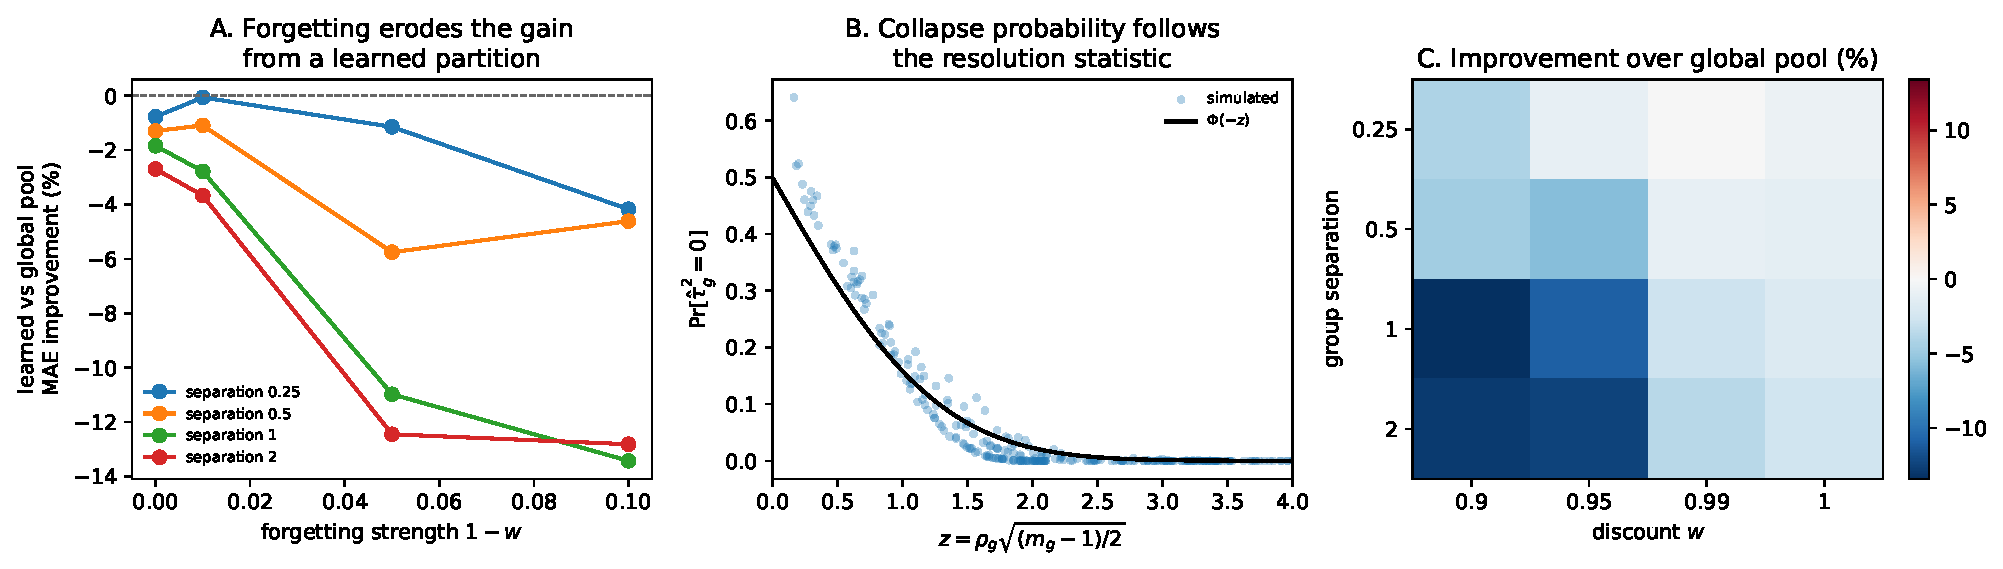
\includegraphics[width=\linewidth]{figs/fig_resolution.pdf}
\caption{Controlled study with known ground truth. \textbf{(A)}
Forgetting raises the leverage of a correct partition: NLL gain of the
true partition over a single pool against forgetting strength
(mean $\pm$ s.e.\ over separations and replicates). \textbf{(B)}
Simulated collapse probability against the resolution statistic
$z=\rho_g\sqrt{(m_g-1)/2}$ (computed from the \emph{true} $\rho_g$,
which the simulation knows), with the predicted $\Phi(-z)$ overlaid;
over $480$ configurations the median absolute error is $0.0006$ and the
$90$th percentile $0.040$, degrading to $0.21$ for small groups that
combine strongly unequal counts with heteroskedastic sampling
variances, where the approximation \emph{understates} collapse.
\textbf{(C)} The gain of the true partition is governed by the item's
own sample size, on every metric: structure held fixed, series length
swept.}
\label{fig:resolution}
\end{figure}

\subsection{When can a partition pay? A one-line diagnostic}
\label{sec:leverage}

The controlled study says the value of a partition is governed by the
credibility weight $\lambda_i=n_i/(n_i+\kappa_g)$. That quantity is
computable from the initialization window alone (one pass for the
sufficient statistics, one EB fit for $\kappa$) before any forecaster is
evaluated, which turns ``should I invest in pooling structure for this
panel?'' from a modeling debate into a measurement.
Table~\ref{tab:leverage} reports it for all five panels, under a single
pool, at $w{=}1$ and at each panel's selected discount.

\begin{table}[t]
\centering
\caption{Credibility leverage under a single pool: median
$\lambda_i=n_i/(n_i+\kappa)$ and the share of items that are
prior-dominated ($\lambda_i<0.1$), at no discounting and at the
panel's selected discount $w^{*}$. Last column: measured MAE effect of
the learned partition relative to the single pool (independent runs,
auto-selected $w$; Appendices~\ref{app:resolution} and~\ref{app:extra}). The only panel whose
median item is prior-dominated at its selected discount is the only
panel where the learned partition wins.}
\label{tab:leverage}
\begin{tabular}{lrrrrr}
\toprule
& & \multicolumn{1}{c}{med.\ $\lambda_i$} & \multicolumn{1}{c}{med.\ $\lambda_i$}
& \multicolumn{1}{c}{$\lambda_i{<}0.1$} & learned vs.\\
panel & $w^{*}$ & ($w{=}1$) & ($w{=}w^{*}$) & ($w{=}w^{*}$) & single pool\\
\midrule
Carparts & $0.90$ & $0.802$ & $\mathbf{0.224}$ & $22.5\%$ & $\mathbf{+2.7\%}$\\
M5 & $0.90$ & $0.996$ & $0.712$ & $18.4\%$ & $-2.3\%$\\
Online Retail & $0.98$ & $0.897$ & $0.749$ & $3.2\%$ & $-2.9\%$\\
RAF & $0.997$ & $0.926$ & $0.917$ & $0.0\%$ & $-13.0\%$\\
Auto & $0.995$ & $0.944$ & $0.942$ & $0.0\%$ & $-3.6\%$\\
\bottomrule
\end{tabular}
\end{table}

Three observations. First, \textbf{the sign of the partition effect
follows the leverage}. Carparts is the only panel whose median item is
prior-dominated at its selected discount, and it is the only panel where
the learned partition beats the single pool. The panels where items own
their estimates ($\lambda_i\approx0.92$--$0.94$) are where it loses
most. (RAF's $-13.0\%$ is inflated by the variance-component collapse.
The regularized run recovers to $-5.0\%$, still negative, consistent
with its high leverage-free share.) Second, \textbf{forgetting is what
creates the leverage that pooling then serves}. Carparts' median
$\lambda_i$ falls from $0.80$ to $0.22$ \emph{because} its selected
discount is aggressive. At $w{=}1$ no panel is prior-dominated. The two
axes are coupled exactly as Proposition~\ref{prop:active} and
Proposition~\ref{prop:twosided} describe: the discount keeps the prior
relevant, and simultaneously determines how much any refinement of that
prior can matter. Third, the table made a \textbf{falsifiable
prediction} that we then tested: M5 has the second-lowest median
leverage ($0.712$, with $18.4\%$ of items prior-dominated), so among the
panels whose median item is \emph{not} prior-dominated, M5 should sit
closest to the sign flip. The M5 partition grid
(Appendix~\ref{app:extra}) is consistent with both halves of the rule.
The median M5 item holds its own estimate and the learned partition
indeed does not pay ($-2.3\%$ MAE against the single pool), and that
deficit is the smallest of the four panels in this group ($-2.3\%$
vs.\ $-2.9\%$ on Online Retail, $-3.6\%$ on Auto, and $-5.0\%$
regularized on RAF). The sign rule survives: only a prior-dominated
median item pays.

\subsection{Sequential (walk-forward) operation}\label{sec:walkforward}

\begin{table}[t]
\centering
\caption{Online Retail, strict walk-forward (7-day blocks; every model
refits or updates per block). The three hierarchical rows differ only in
the forgetting configuration. Probabilistic walk-forward results are in
Appendix~\ref{app:extra}.}
\label{tab:walkforward}
\small
\setlength{\tabcolsep}{5pt}
\begin{tabular}{lccc}
\toprule
Model & MAE & RMSE & RMSSE\\
\midrule
CrostonClassic & 5.692 & 16.937 & 4.854\\
CrostonSBA & 5.586 & 16.931 & 4.836\\
TSB & 5.434 & 17.754 & 4.815\\
ADIDA & \best{5.320} & \best{16.728} & \secondbest{4.637}\\
IMAPA & \secondbest{5.332} & \secondbest{16.745} & \best{4.632}\\
AutoARIMA & 5.482 & 16.904 & 5.105\\
AutoTheta & 5.394 & 16.836 & 4.735\\
\midrule
Stationary configuration ($w{=}1$) & 5.586 & 17.260 & 4.725\\
Forgetting configuration (tax., $0.95$) & 5.411 & 17.059 & 4.682\\
\REMIX{} (online) & 5.474 & 17.244 & 4.761\\
\bottomrule
\end{tabular}
\end{table}

Fixed-origin evaluation isolates stable intensity estimation, but real
deployments update sequentially. Table~\ref{tab:walkforward} runs a
strict block-wise walk-forward protocol in which every baseline refits
each block and the hierarchical models update online sufficient
statistics without refitting. Forgetting improves walk-forward MAE in
both configurations we test: the \REMIX{}-selected pair (mixture,
$w{=}0.98$) improves MAE $5.586\!\to\!5.474$ but concedes RMSSE
($4.725\!\to\!4.761$): its per-block occurrence discounting, layered on
the discounted initialization, trades some scaled-error stability for
responsiveness, while the stronger-forgetting configuration (taxonomy,
$w{=}0.95$) improves both metrics ($5.411$/$4.682$), closing most of the
gap to the temporal-aggregation leaders, which are strongest precisely
in this regime because per-block refits give them their own form of
adaptation. That the fixed-origin selector picks a milder discount than
walk-forward would reward is another instance of the
criterion-alignment point of Section~\ref{sec:limitations}.

\begin{table}[t]
\centering
\caption{Online Retail, \textbf{probabilistic walk-forward}: scaled
pinball by quantile and mean, and 80\% coverage, marginal and on
positive-demand observations (Cov$^{+}$), under identical block-wise
updating (\REMIX{} raw law with online sufficient-statistics updates;
wrappers refit per block). The wrappers reach near-nominal marginal
coverage by covering the zeros; where demand actually occurs their
intervals cover under half.}
\label{tab:wfprob}
\small
\setlength{\tabcolsep}{2.9pt}
\begin{tabular}{lcccccccc}
\toprule
Model & q10 & q25 & q50 & q75 & q90 & Mean & Cov@80 & Cov$^{+}$@80\\
\midrule
CP-Croston & 0.341 & 0.778 & 1.364 & 1.745 & 2.632 & 1.372 & 0.793 & 0.479\\
CP-SBA & 0.334 & 0.762 & 1.343 & 1.725 & 2.722 & 1.377 & 0.793 & 0.482\\
CP-TSB & 0.451 & 0.899 & 1.289 & 1.385 & 2.842 & 1.373 & 0.795 & 0.468\\
CP-ADIDA & \secondbest{0.277} & \secondbest{0.627} & \secondbest{1.050} & \best{1.319} & \secondbest{2.514} & \secondbest{1.158} & 0.791 & 0.473\\
CP-IMAPA & 0.292 & 0.660 & 1.084 & 1.329 & 2.522 & 1.177 & 0.791 & 0.471\\
\midrule
\REMIX{} (online) & \best{0.183} & \best{0.458} & \best{0.910} & \secondbest{1.327} & \best{1.460} & \best{0.868} & 0.899 & 0.611\\
\bottomrule
\end{tabular}
\end{table}

The probabilistic picture under walk-forward is where the model family
pays most (Table~\ref{tab:wfprob}). \REMIX{}'s predictive law is best at
four of five quantiles (at q75 it trails CP-ADIDA by $0.6\%$) and beats
the best conformal wrapper by $25\%$ on mean SPL; at the
inventory-critical q90 the margin is $42\%$. The coverage columns say
why: per-block refitting lets the wrappers hold near-nominal
\emph{marginal} coverage, but they do it by covering the zeros. On the
observations where demand actually occurs, their $80\%$ intervals cover
$47$--$48\%$, versus $61\%$ for the hierarchical law. The point-forecast
gap to the temporal-aggregation leaders
(Table~\ref{tab:walkforward}) buys a distribution the wrappers do not
match in the protocol closest to deployment.

\paragraph{Is stale selection the problem? A re-selection experiment.}
We tested online re-selection directly, in a full-refit variant of the
protocol: every arm refits the closed-form model on all revealed data
each block (still seconds per block), and the arms differ only in how
often the joint $(g,w)$ selection is re-run. Selecting once at the
origin gives MAE $5.372$ / RMSSE $4.692$; re-selecting every four
blocks gives $5.408$/$4.655$, and every block $5.405$/$4.647$, at
$7\times$ and $27\times$ the selection compute. Two readings. First,
full per-block refitting alone (versus the online sufficient-statistics
updates of Table~\ref{tab:walkforward}) improves \REMIX{}'s walk-forward
MAE from $5.474$ to $5.372$, closing most of the distance to the
temporal-aggregation leaders. Second, the re-selection trajectory says
what adaptation is actually worth: the structure is re-picked
essentially always (mixture in 35 of 36 selections), while the selected
discount strengthens monotonically from $0.98$ through $0.95$ to $0.90$
as the drift-era data enters the window, exactly the direction the
criterion-alignment reading predicts. Acting on that drift buys about
$1\%$ of RMSSE at a $0.6\%$ MAE cost. Stale selection is not the
missing lever.

\subsection{Statistical significance and uncertainty quality}
\label{sec:significance}

\begin{table}[t]
\centering
\caption{Paired per-series tests on Online Retail (3{,}649 series):
forgetting configuration vs.\ each alternative on per-series MAE.
Negative favors forgetting; $p$-values Holm-adjusted. On per-series RMSE
the forgetting configuration beats \emph{every} baseline at $p<0.005$.}
\label{tab:significance}
\small
\setlength{\tabcolsep}{5pt}
\begin{tabular}{lccc}
\toprule
vs. & Mean diff & $p_t$ & $p_{\mathrm{Wilcoxon}}$\\
\midrule
Stationary hierarchical & $-0.234$ & $<\!10^{-24}$ & $<\!10^{-7}$\\
TSB & $-0.110$ & $0.083$ & $<\!10^{-166}$\\
TSB-tuned & $-0.159$ & $1.1\times10^{-4}$ & $<\!10^{-71}$\\
ADIDA & $-0.105$ & $1.1\times10^{-4}$ & $<\!10^{-71}$\\
IMAPA & $-0.118$ & $<\!10^{-4}$ & $<\!10^{-85}$\\
CrostonSBA & $-0.941$ & $<\!10^{-29}$ & $<\!10^{-58}$\\
AutoARIMA & $-0.959$ & $<\!10^{-15}$ & $<\!10^{-5}$\\
AutoTheta & $-2.713$ & $<\!10^{-83}$ & $<\!10^{-99}$\\
\bottomrule
\end{tabular}
\end{table}

\begin{table}[t]
\centering
\caption{Raw \REMIX{} interval quality across the five panels (nominal
80\%). Mild over-coverage is the expected signature of the log-normal
tail on sparse counts; the optional calibration layer trades it toward
nominal at 11\% narrower width (Section~\ref{sec:main-results}).}
\label{tab:coverage}
\small
\setlength{\tabcolsep}{4.6pt}
\begin{tabular}{lccccc}
\toprule
 & OR & M5 & Auto & Carparts & RAF\\
\midrule
Coverage@80 & 0.896 & 0.830 & 0.859 & 0.910 & 0.922\\
AIW@80 & 10.34 & 2.58 & 9.41 & 1.23 & 0.76\\
\bottomrule
\end{tabular}
\end{table}

Table~\ref{tab:significance} confirms the ablation's headline is
systematic rather than incidental: the forgetting configuration improves
per-series MAE over the stationary model at $p<10^{-24}$ and is never
significantly worse than any baseline on either metric. The two-sided
cases are TSB and TSB-tuned, whose median-series MAE is marginally
better while their loss tails are far heavier, consistent with
Table~\ref{tab:ablation},
where TSB's RMSE is worst among all hierarchical configurations; on
per-series RMSE the forgetting configuration beats TSB-tuned on both
mean and median.
Table~\ref{tab:coverage} reports interval quality: against the nominal
$0.80$, raw coverage lies in $[0.830, 0.922]$ with no tuning: M5 sits
nearly on target, while RAF's $0.922$ is the largest deviation
(its very short intervals, AIW $0.76$, make the discrete zero mass
dominate). Section~\ref{sec:limitations} discusses this over-coverage
explicitly.

\paragraph{Cross-dataset comparison (descriptive).} Figure~\ref{fig:cd}
ranks per-series scaled squared errors (the RMSSE numerator) over all
$16{,}833$ rankable series from the five panels. We report it as a
\emph{descriptive} summary, not as a hypothesis test, because the
standard Friedman--Nemenyi protocol blocks on \emph{datasets} whereas we
block on series: with five panels contributing between $2{,}509$ and
$5{,}000$ series each, the pooled ranking is dominated by the larger
panels and the blocks are not exchangeable. A per-dataset rank table is
in Appendix~\ref{app:extra}, and the ordering there is the same. Read
descriptively, the temporal-aggregation methods lead the \emph{typical}
series narrowly (\REMIX{} sits within the critical-difference band of
IMAPA and $0.09$ average-rank behind ADIDA at $\mathrm{CD}=0.08$), while
TSB, the MAE champion of Table~\ref{tab:point}, ranks \emph{last}: rank
statistics weight every series equally, and zero-leaning forecasts pay on
the series that matter. Diebold--Mariano-style paired tests on the same
per-series losses give \REMIX{} an advantage in $25$ of $35$
dataset$\times$baseline comparisons and a disadvantage in $2$ (IMAPA on
Carparts, ADIDA on RAF), matching the two panels where
Table~\ref{tab:point} already showed it trailing. DM was designed for two
competing forecasts of one series. Applying it to per-series aggregate
losses across a panel is a common but non-standard use, so we treat the
counts as effect-size summaries rather than as a family of tests with
controlled error.

\begin{figure}[t]
\centering
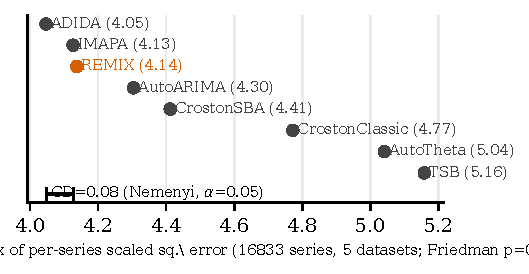
\includegraphics[width=0.93\linewidth]{figs/cd_diagram.pdf}
\caption{Average ranks of per-series scaled squared errors across all
five panels, with the Nemenyi critical difference drawn at
$\alpha{=}0.05$ for scale. Lower is better. Descriptive: the blocks here
are series, not datasets, so this is not a valid Friedman--Nemenyi test
(Section~\ref{sec:significance}).}
\label{fig:cd}
\end{figure}

\subsection{The criterion the selector is given}\label{sec:criterion}
Nothing in the selector is tied to pinball loss. It scores whatever
criterion it is handed on the same validation split. That makes the
choice of criterion a deployment decision rather than a property of the
model, and it has a measurable cost when the criterion and the reported
metric disagree. On Online Retail, selecting by validation \emph{MAE}
instead of scaled pinball picks (global pool, $w{=}0.90$) rather than
(mixture, $w{=}0.98$), and that configuration attains out-of-sample MAE
$5.5083$: better than every configuration in
Table~\ref{tab:ablation} and every baseline in Table~\ref{tab:point},
including TSB's $5.5736$. The pinball-selected configuration reaches
$5.6639$. So the $1.6\%$ MAE gap to TSB reported in
Section~\ref{sec:experiments} is a consequence of selecting on a
distributional criterion, not a limit of the model family: a deployment
that cares about MAE can have the better MAE by asking for it.

We report this as a two-sided fact. It supports the design (the selector
is objective-aware), and it also means our headline configuration is not
the MAE-optimal member of its own family. A full cross-objective study
(selecting under mean SPL, MAE, RMSSE, q90 pinball, and a newsvendor cost,
then reporting the regret matrix across all five metrics and all five
panels) is the natural completion and is not run here.

\paragraph{Robustness of the selector.} Beyond the validation-ratio
sweep of Section~\ref{sec:selector}, the conjugate variance prior
$\nu$ barely moves the probabilistic results
(mean SPL $0.8841/0.8841/0.8843/0.8844$ for $\nu\in\{5,10,20,50\}$ on
Online Retail, coverage varying by less than $0.2$ points), matching the
stability one expects from a conjugate variance prior with moderate
degrees of freedom. Halving the discount grid to five points never changes the
selected structure on any panel and moves $w$ only to the nearest
neighboring grid point on two of the five. The selector is doing coarse
structural triage, and coarse triage is stable.

\subsection{Efficiency}\label{sec:efficiency}
On Online Retail (CPU): the base fit-plus-predict is $0.3$\,ms/series;
full \REMIX{} selection (24 candidate fits) $6$\,ms/series; AutoARIMA
$19$\,ms/series; neural baselines are orders of magnitude slower at equal
or worse accuracy (Appendix~\ref{app:extra}). Determinism makes results
bit-reproducible without seeds.

% =========================================================================
\section{Limitations}\label{sec:limitations}
% =========================================================================
We group the boundaries of this study into four kinds.

\paragraph{Model distribution and calibration.}
\textbf{(1)}~The log-normal size law keeps every update closed form but
its tail can be conservative on panels with heavy-tailed spikes:
Carparts' q90 favors AutoTheta and M5's q90 favors conformal wrappers
even though \REMIX{} wins both means (on Carparts the ordering reverses
back in \REMIX{}'s favor from $q{=}0.95$ on,
Appendix~\ref{app:fartail}). A Gamma size block (conjugate in
the same architecture) is the natural next instantiation.
\textbf{(2)}~Raw intervals over-cover on the sparsest panels (up to
$0.922$ against nominal $0.80$ on RAF, Table~\ref{tab:coverage}), and on
RAF the standard quantile levels saturate: the all-zero forecast attains
a marginally lower mean SPL than every method there. The far-tail
levels ($q\ge0.95$) resolve this (Appendix~\ref{app:fartail}); CRPS and
a cost-based criterion remain unrun.

\paragraph{Assumptions behind the resolution condition.}
\textbf{(3)}~Corollary~\ref{cor:resolution} is stated under the Gaussian
working model for the item means and uses a $\chi^2$ approximation for
$S_g^2$. Section~\ref{sec:synthetic} shows the approximation is accurate
except for small groups that combine strongly unequal counts with
strongly unequal sampling variances, where it \emph{under}-states the
collapse probability by up to $0.21$. Read it as a calibrated
order-of-magnitude threshold, not an exact test. It is an
estimator-specific estimability statement, not an information-theoretic
impossibility result, and it says nothing about which partition is best
\emph{below} the threshold. Whether a partition learned under a
different objective (for instance one maximizing between-group
separation subject to keeping $\rho_g\sqrt{m_g}$ above threshold) would
do better is open, and is the experiment we would run next.
\textbf{(4)}~The mixture assignment is hard. A
soft-responsibility predictive mixture is a strict generalization that
would add one matrix multiply. It is also the one extension not covered
by our negative result: mixing over components changes the \emph{shape}
of the predictive distribution rather than only the prior it shrinks
toward, so it is not bounded by Corollary~\ref{cor:resolution} in the
same way, and it targets the upper quantiles where
Table~\ref{tab:prob} shows our remaining weakness. \textbf{(5)}~Hyperparameter uncertainty
enters only through bootstrap averaging of the EB fit, not full posterior
propagation.

\paragraph{Baseline and inference scope.}
\textbf{(6)}~We do not compare directly against external
hierarchical Bayesian implementations
\citep{chapados2014,seeger2016,pitkin2024}: they require sampling or
variational machinery whose faithful reproduction at our scale was out
of budget, so our hierarchical comparisons are internal (the $w{=}1$
column of the ablation) plus iETS as the likelihood-based state-space
representative. Claims about those methods are limited to their
published computational profiles. In particular we have not run a
dynamic hierarchical hurdle or discount-factor Bayesian model, so we do
not characterize that family empirically. Appendix~\ref{app:mcmc}
closes the inference-method half of this gap: a full-posterior Gibbs
sampler for model \eqref{eq:model} itself matches the closed-form
pipeline within $1\%$ on every metric on a 500-series subsample, so the
EB approximation is not the accuracy bottleneck; the model-class half
(richer external samplers) remains open. \textbf{(7)}~Our Tweedie
baseline is a per-series autoregressive GLM. The GP-based Tweedie method
of \citet{damato2025}, whose Auto/Carparts/RAF protocol we adopt, is
\emph{not} run here (its per-series GP training was outside our compute
budget), so we make no claim about its accuracy relative to ours.
\textbf{(8)}~The conformal comparison uses one static split-conformal
construction. Adaptive and weighted variants designed for nonstationarity
are not evaluated. \textbf{(9)}~The Deep Renewal Process comparison could
not be re-executed in the current environment (unmaintained MXNet
dependency) and is reported as indicative only.

\paragraph{Criterion and deployment alignment.}
\textbf{(10)}~The selection criterion is a single pinball-based score.
Section~\ref{sec:criterion} shows the selector tracks whichever criterion
it is given, but a full cross-objective study (including an inventory
cost criterion) is left to future work.
\textbf{(11)}~The discount is selected under the fixed-origin protocol
and reused in walk-forward. We keep the initialization discount and the
online block update distinct and do not compound them. The re-selection
experiment of Section~\ref{sec:walkforward} bounds what online
re-selection is worth on Online Retail (about $1\%$ RMSSE for $0.6\%$
MAE at $7$--$27\times$ selection compute); the headline walk-forward
numbers remain the fixed-origin configuration operated sequentially.

% =========================================================================
\section{Conclusion}\label{sec:conclusion}
% =========================================================================
How to pool across items and how to forget across time are the two
structural decisions of intermittent-demand forecasting, and neither
needs to be hard-coded: \REMIX{} selects both by chronological validation
inside a closed-form empirical-Bayes family whose noninformative corner
is exactly classical TSB, and leads mean scaled pinball among
non-degenerate methods on all five public panels while running in
milliseconds per item. The lead is largest exactly where a forecaster
earns its keep: under strict walk-forward updating (25\% over the best
conformal wrapper, with honest coverage where demand actually occurs)
and in the far tail, where the zero forecast's apparent advantage
collapses. Full-posterior sampling of the same hierarchy changes no
metric by more than $1\%$, so the closed form gives up essentially
nothing to the inference approximation while keeping bit-reproducible,
diagnostics-free estimation.

The finding we consider most useful is asymmetric, and each half of it
has a mechanism. Forgetting is the first-order driver of accuracy, and
its theory ($\delta^{2/3}$ tracking, always-active shrinkage) predicts
the selector's behavior. Refining the pooling partition is second-order
on aggregate metrics, not because structure is absent or unrecoverable,
but because its value is bounded by the credibility leverage
$1-\lambda_i$, which on most public panels is small: items hold their
own histories. The two halves are coupled. The discount that tracks
drift is the same quantity that shrinks effective samples, raising the
prior's leverage while degrading the resolution with which a fine
partition can be estimated (Proposition~\ref{prop:twosided}). Which
effect wins is an empirical question the leverage table answers per
panel, before any forecaster is run. On the one panel whose median item
is prior-dominated, the learned partition does win.

Two warnings travel beyond this model family. Mean absolute error
reverses the ranking of a structure known to be correct in our
controlled study, and rewards the all-zero forecast on three of five
real panels. Rankings of intermittent-demand methods built on it should
be read accordingly. And plug-in variance components collapse under
recency weighting: any method that combines discounting with
hierarchical shrinkage inherits that failure mode, along with the
one-line regularization that removes it.

Natural extensions: soft component responsibilities (the one change our
resolution analysis does not bound, and aimed at the far quantiles),
covariates via mixed-effects links, Gamma size laws, cost-aware
selection criteria tied to service levels, and partition objectives
that maximize post-shrinkage separation subject to the resolution
condition: the experiment our diagnostic most directly motivates.

% =========================================================================
\section*{Reproducibility Statement}
All five datasets are public (UCI 352; Kaggle M5-Accuracy; the gluon-ts
\texttt{intermittent-datasets} branch for Auto and RAF; Zenodo record
4656022 for Carparts). Conversion and preprocessing scripts are included
in the released code. The full pipeline is deterministic (closed-form
EB, seed-free quantile-based EM initialization), so no seed policy is
required for the forecaster itself (the only stochastic elements are the
seed-controlled M5 subsample and the $B{=}20$ bootstrap, both fixed at
seed 42), and an automated test asserts that two end-to-end runs are
bit-identical. Every table maps to one experiment directory via a
manifest file, and each run writes its selection diagnostics (chosen
partition, discount, BIC curves) alongside its metrics. Hardware and
timing methodology are specified in Appendix~\ref{app:implementation}.
The complete experiment suite runs on one CPU workstation in under a
day, dominated by the statistical baselines rather than \REMIX{}. An
anonymized code repository will accompany the submission.

\begin{thebibliography}{99}

\bibitem[B\"uhlmann(1967)]{buhlmann1967}
H.~B\"uhlmann.
\newblock Experience rating and credibility.
\newblock \emph{ASTIN Bulletin}, 4(3):199--207, 1967.

\bibitem[Chapados(2014)]{chapados2014}
N.~Chapados.
\newblock Effective Bayesian modeling of groups of related count time series.
\newblock In \emph{ICML}, 2014.

\bibitem[Chen(2015)]{chen2015}
D.~Chen.
\newblock Online Retail dataset, UCI Machine Learning Repository, 2015.

\bibitem[Croston(1972)]{croston1972}
J.~D. Croston.
\newblock Forecasting and stock control for intermittent demands.
\newblock \emph{Operational Research Quarterly}, 23(3):289--303, 1972.

\bibitem[Damato et~al.(2025)]{damato2025}
S.~Damato, D.~Azzimonti, and G.~Corani.
\newblock Forecasting intermittent time series with Gaussian processes and
  Tweedie likelihood.
\newblock \emph{International Journal of Forecasting}, 2025.

\bibitem[Gibbs and Cand\`es(2021)]{gibbs2021}
I.~Gibbs and E.~Cand\`es.
\newblock Adaptive conformal inference under distribution shift.
\newblock In \emph{NeurIPS}, 2021.

\bibitem[Gneiting and Raftery(2007)]{gneiting2007}
T.~Gneiting and A.~E. Raftery.
\newblock Strictly proper scoring rules, prediction, and estimation.
\newblock \emph{JASA}, 102(477):359--378, 2007.

\bibitem[Ibrahim and Chen(2000)]{ibrahimchen2000}
J.~G. Ibrahim and M.-H. Chen.
\newblock Power prior distributions for regression models.
\newblock \emph{Statistical Science}, 15(1):46--60, 2000.

\bibitem[Keribin(2000)]{keribin2000}
C.~Keribin.
\newblock Consistent estimation of the order of mixture models.
\newblock \emph{Sankhy\=a A}, 62(1):49--66, 2000.

\bibitem[Kolassa(2016)]{kolassa2016}
S.~Kolassa.
\newblock Evaluating predictive count data distributions in retail sales
  forecasting.
\newblock \emph{International Journal of Forecasting}, 32(3):788--803, 2016.

\bibitem[Kourentzes and Petropoulos(2016)]{kourentzes2016}
N.~Kourentzes and F.~Petropoulos.
\newblock Forecasting with multivariate temporal aggregation.
\newblock \emph{Int.\ J.\ Production Economics}, 181:145--153, 2016.

\bibitem[Lei et~al.(2018)]{lei2018}
J.~Lei, M.~G'Sell, A.~Rinaldo, R.~J. Tibshirani, and L.~Wasserman.
\newblock Distribution-free predictive inference for regression.
\newblock \emph{JASA}, 113(523):1094--1111, 2018.

\bibitem[Makridakis et~al.(2022)]{makridakis2022}
S.~Makridakis, E.~Spiliotis, and V.~Assimakopoulos.
\newblock M5 accuracy competition: Results, findings, and conclusions.
\newblock \emph{International Journal of Forecasting}, 38(4):1346--1364, 2022.

\bibitem[Montero-Manso and Hyndman(2021)]{monteromanso2021}
P.~Montero-Manso and R.~J. Hyndman.
\newblock Principles and algorithms for forecasting groups of time
  series: Locality and globality.
\newblock \emph{International Journal of Forecasting}, 37(4):1632--1653,
  2021.

\bibitem[Nikolopoulos et~al.(2011)]{nikolopoulos2011}
K.~Nikolopoulos, A.~A. Syntetos, J.~E. Boylan, F.~Petropoulos, and
  V.~Assimakopoulos.
\newblock An aggregate--disaggregate intermittent demand approach (ADIDA).
\newblock \emph{JORS}, 62(3):544--554, 2011.

\bibitem[Pitkin et~al.(2024)]{pitkin2024}
J.~Pitkin, I.~Manolopoulou, and G.~Ross.
\newblock Bayesian hierarchical modelling of sparse count processes in
  retail analytics.
\newblock \emph{Annals of Applied Statistics}, 18(2):946--965, 2024.

\bibitem[Salinas et~al.(2020)]{salinas2020}
D.~Salinas, V.~Flunkert, J.~Gasthaus, and T.~Januschowski.
\newblock DeepAR: Probabilistic forecasting with autoregressive recurrent
  networks.
\newblock \emph{International Journal of Forecasting}, 36(3):1181--1191, 2020.

\bibitem[Seeger et~al.(2016)]{seeger2016}
M.~Seeger, D.~Salinas, and V.~Flunkert.
\newblock Bayesian intermittent demand forecasting for large inventories.
\newblock In \emph{NeurIPS}, 2016.

\bibitem[Snyder et~al.(2012)]{snyder2012}
R.~D. Snyder, J.~K. Ord, and A.~Beaumont.
\newblock Forecasting the intermittent demand for slow-moving
  inventories: A modelling approach.
\newblock \emph{International Journal of Forecasting}, 28(2):485--496,
  2012.

\bibitem[Svetunkov and Boylan(2023)]{svetunkov2023iets}
I.~Svetunkov and J.~E. Boylan.
\newblock iETS: State space model for intermittent demand forecasting.
\newblock \emph{Int.\ J.\ Production Economics}, 265, 2023.

\bibitem[Syntetos and Boylan(2005)]{syntetos2005accuracy}
A.~A. Syntetos and J.~E. Boylan.
\newblock The accuracy of intermittent demand estimates.
\newblock \emph{International Journal of Forecasting}, 21(2):303--314, 2005.

\bibitem[Syntetos et~al.(2005)]{syntetos2005categorization}
A.~A. Syntetos, J.~E. Boylan, and J.~D. Croston.
\newblock On the categorization of demand patterns.
\newblock \emph{JORS}, 56(5):495--503, 2005.

\bibitem[Teunter et~al.(2011)]{teunter2011}
R.~H. Teunter, A.~A. Syntetos, and M.~Z. Babai.
\newblock Intermittent demand: Linking forecasting to inventory
  obsolescence.
\newblock \emph{EJOR}, 214(3):606--615, 2011.

\bibitem[West and Harrison(1997)]{westharrison1997}
M.~West and J.~Harrison.
\newblock \emph{Bayesian Forecasting and Dynamic Models}.
\newblock Springer, 2nd edition, 1997.

\bibitem[T\"urkmen et~al.(2019)]{turkmen2019}
A.~C. T\"urkmen, Y.~Wang, and T.~Januschowski.
\newblock Intermittent demand forecasting with deep renewal processes.
\newblock \emph{arXiv:1911.10416}, 2019.

\end{thebibliography}

% =========================================================================
\appendix
\onecolumn

\section{Notation}\label{app:notation}

\begin{table}[h]
\centering
\small
\begin{tabular}{ll}
\toprule
$y_{i,t}$, $p_{i,t}$, $\ell_{i,t}$ & demand, occurrence indicator, log-size\\
$T_i$ & initialization-window length of item $i$\\
$g(i)$, $K$ & pooling group of item $i$; number of mixture components\\
$\alpha_g,\beta_g$ & Beta occurrence prior; $\phi_g=\alpha_g+\beta_g$ its strength\\
$\mu_{0,g},\tau^2_g,\sigma^2_g$ & size prior location, between/within-item variances\\
$w$; $b$ & recency discount; forgetting strength $b=1-w$\\
$n_i(w), s_i(w)$ & discounted observation / occurrence pseudo-counts\\
$\bar p_i(w)$ & discounted empirical occurrence rate $s_i(w)/n_i(w)$\\
$\lambda_i(w)$ & credibility weight $n_i(w)/(n_i(w)+\phi_g)$\\
$\hat\pi_i,\hat\mu_i,\hat\sigma^2_i$ & posterior means of occurrence, log-size, variance\\
$\alpha_p$ & classical TSB occurrence smoothing constant ($=1-w$)\\
$\delta$ & occurrence drift rate (Proposition~\ref{prop:drift})\\
$M$, $n$ & candidate count and validation size (Prop.~\ref{prop:oracle})\\
$B$ & bootstrap draws for hyperparameter averaging\\
\bottomrule
\end{tabular}
\end{table}

\section{Proofs}\label{app:proofs}

\subsection{Proof of Proposition~\ref{prop:tsb-limit}}
(i) Immediate from \eqref{eq:disc-post} since $s(w),n(w)$ are finite.
(ii) Induction: $\hat p_1=(1-w)p_1+w\hat p_0$. If the closed form holds at
$T-1$, then
$\hat p_T=(1-w)p_T+w\hat p_{T-1}=(1-w)\sum_{t=1}^{T}w^{T-t}p_t+w^{T}\hat p_0$.
With $n(w)=(1-w^{T})/(1-w)$,
\[
\bar p(w)=\frac{(1-w)\sum_t w^{T-t}p_t}{1-w^{T}}
=\frac{\hat p_T-w^{T}\hat p_0}{1-w^{T}}.
\]
(iii) Rearranging, $\bar p(w)-\hat p_T=w^{T}(\bar p(w)-\hat p_0)$, and
$|\bar p(w)-\hat p_0|\le1$. \qed

\subsection{Proof of Proposition~\ref{prop:active}}
$n(w)=(1-w^{T})/(1-w)\le1/(1-w)$ and $x\mapsto x/(x+\phi)$ is increasing,
so $\lambda(w)\le[1/(1-w)]/[1/(1-w)+\phi]=1/(1+(1-w)\phi)$. \qed

\subsection{Proof of Proposition~\ref{prop:drift} and
Corollary~\ref{cor:rate}}
With $k=T-t$ and $\sum_{k\ge0}kw^k=w/(1-w)^2$,
\[
\bigl|\E\bar p(w)-\pi_T\bigr|
=\Bigl|\frac{\sum_t w^{T-t}(\pi_t-\pi_T)}{n(w)}\Bigr|
\le\frac{\delta\,w/(1-w)^2}{(1-w^{T})/(1-w)}
=\delta\,\frac{w}{(1-w)(1-w^{T})}.
\]
By independence and $\pi_t(1-\pi_t)\le\tfrac14$,
\[
\Var\,\bar p(w)\le\frac{\tfrac14\,(1-w^{2T})/(1-w^{2})}
{[(1-w^{T})/(1-w)]^{2}}
=\frac14\cdot\frac{(1-w)(1+w^{T})}{(1+w)(1-w^{T})}.
\]
Decomposing
$\hat\pi-\pi_T=\lambda(\bar p-\E\bar p)+\lambda(\E\bar p-\pi_T)+(1-\lambda)(\mu_\pi-\pi_T)$,
the first term is zero-mean and independent of the deterministic
remainder, giving
$\E(\hat\pi-\pi_T)^2\le[\lambda\mathrm{B}(w)+(1-\lambda)|\mu_\pi-\pi_T|]^2
+\lambda^2\Var\bar p(w)$ with $\mathrm{B}(w)$ the bias bound. For the
corollary set $b=1-w$ and let $T\to\infty$ (so $w^{T}\to0$): the squared
bias bound behaves as $\delta^2(1-b)^2/b^2\sim\delta^2/b^2$ and the
variance bound becomes $\tfrac14\, b/(2-b)$, which is $b/8$ to leading
order as $b\to0$. Minimizing $f(b)=\delta^2/b^2+b/8$ gives
$f'(b)=-2\delta^2/b^3+1/8=0$, i.e.,
$b^{*}=(16\delta^{2})^{1/3}=2^{4/3}\delta^{2/3}$, and
$f(b^{*})=O(\delta^{2/3})$. \qed

\subsection{Proof of Proposition~\ref{prop:oracle}}
For each candidate $c$, Hoeffding's inequality for independent scores in
$[0,B]$ gives
$\Pr\bigl(|\hat R(c)-R(c)|>t\bigr)\le2\exp(-2nt^2/B^2)$. A union bound
over the $M$ candidates makes
$\sup_c|\hat R(c)-R(c)|\le t$ hold with probability at least
$1-2M\exp(-2nt^2/B^2)$. Setting the right side to $\eta$ yields
$t=B\sqrt{\log(2M/\eta)/(2n)}$. On this event,
$R(\hat c)\le\hat R(\hat c)+t\le\hat R(c^{*})+t\le R(c^{*})+2t$ with
$c^{*}=\arg\min_c R(c)$, which is the claim with constant
$2t=B\sqrt{2\log(2M/\eta)/n}$. \qed

\subsection{Proof of Proposition~\ref{prop:credibility}}
With known $(\alpha_g,\beta_g)$ and $s_i\mid\pi_i\sim
\mathrm{Bin}(n_i,\pi_i)$, $\pi_i\sim\mathrm{Beta}(\alpha_g,\beta_g)$,
the posterior mean $\hat\pi_i=\lambda_i\bar p_i+(1-\lambda_i)\mu_\pi$
with $\lambda_i=n_i/(n_i+\phi_g)$ minimizes Bayes risk under squared
loss among all estimators (tower property). Restricting to linear
combinations $a\bar p_i+b$, the Bayes risk is
$a^2\,\E[\Var(\bar p_i\mid\pi_i)] + (1-a)^2\Var(\pi_i)$ at the optimal
intercept, minimized at
$a^{*}=\Var(\pi_i)/\bigl(\Var(\pi_i)+\E[\Var(\bar p_i\mid\pi_i)]\bigr)
=\lambda_i$, the B\"uhlmann credibility weight. The minimum is strictly
below the risk of $a=1$ (the empirical rate) whenever
$\Var(\pi_i)<\infty$ and $\phi_g>0$. \qed

\subsection{Proof of Proposition~\ref{prop:twosided} and
Corollary~\ref{cor:resolution}}

\textbf{(i)} $\lambda_i=n_i/(n_i+\kappa_g)$ is increasing in $n_i$, and
$n_i\le\sum_{k\ge0}w^{k}=(1-w)^{-1}$ for $w<1$. Substituting the bound,
$\lambda_i\le\frac{(1-w)^{-1}}{(1-w)^{-1}+\kappa_g}
=\bigl[1+(1-w)\kappa_g\bigr]^{-1}$, which is $<1$ whenever $w<1$ and
$\kappa_g>0$.

\textbf{(ii)} Write $\bar y_i=\mu_i+e_i$ with
$\mu_i\sim N(\mu_g,\tau_g^2)$ and $e_i\sim N(0,s_i)$ independent,
$s_i=\sigma_g^2/n_i$, so $\Var(\bar y_i)=\tau_g^2+s_i$. For the sample
variance $S_g^2=(m_g-1)^{-1}\sum_{i\in g}(\bar y_i-\bar{\bar y})^2$,
independence gives
$\Var(\bar{\bar y})=m_g^{-2}\sum_i(\tau_g^2+s_i)$ and hence
\[
\E[S_g^2]=\frac{\sum_i(\tau_g^2+s_i)-m_g\Var(\bar{\bar y})}{m_g-1}
=\frac{(1-m_g^{-1})\sum_i(\tau_g^2+s_i)}{m_g-1}
=\tau_g^2+\bar s_g ,
\]
exactly, with no balance assumption. The estimator truncates precisely
when $S_g^2\le\bar s_g$. Under the working model $S_g^2$ is
approximately $(\tau_g^2+\bar s_g)\chi^2_{m_g-1}/(m_g-1)$, so
$\Var(S_g^2)\simeq\frac{2}{m_g-1}(\tau_g^2+\bar s_g)^2$ and the
standardized distance from the truncation boundary is
\[
\frac{\E[S_g^2]-\bar s_g}{\sqrt{\Var(S_g^2)}}
=\frac{\tau_g^2}{\sqrt{2/(m_g-1)}\,(\tau_g^2+\bar s_g)}
=\sqrt{\tfrac{m_g-1}{2}}\;\rho_g ,
\]
giving the stated normal approximation for
$\Pr[S_g^2\le\bar s_g]$. The discount bound follows from
$n_i\le(1-w)^{-1}$: $s_i=\sigma_g^2/n_i\ge(1-w)\sigma_g^2$ for every
$i$, hence $\bar s_g\ge(1-w)\sigma_g^2$, and $\rho_g$ is decreasing in
$\bar s_g$. Finally $\hat\tau_g^2=0$ gives $\kappa_g=\infty$ and
$\lambda_i=0$.

\textbf{(iii)} $\tilde\tau_g^2\ge(1-\omega_g)\hat\tau_0^2$ because
$\hat\tau_g^2\ge0$ and $\omega_g\in[0,1)$. Then
$\tilde\kappa_g=\sigma_g^2/\tilde\tau_g^2\le
\sigma_g^2/[(1-\omega_g)\hat\tau_0^2]$, and monotonicity of
$\lambda_i$ in $\kappa_g$ gives the bound, which is strictly positive
for any $n_i>0$.

\textbf{Corollary.} Requiring the collapse probability to stay below a
fixed level is, by (ii), the condition $\rho_g\sqrt{(m_g-1)/2}\ge c$ for
a constant $c$ of order one. Solving
$\rho_g=\tau_g^2/(\tau_g^2+\bar s_g)\ge c\sqrt{2/(m_g-1)}$ for
$\tau_g^2$ gives
$\tau_g^2\ge\bar s_g\,c\sqrt{2}/(\sqrt{m_g-1}-c\sqrt2)$, i.e.\ the
stated order $\bar s_g/(\sqrt{m_g-1}-1)$ up to the constant. Refining a
partition decreases $m_g$ and, by construction of the mixture objective,
$\tau_g^2$, while decreasing $w$ raises the floor $(1-w)\sigma_g^2$ on
$\bar s_g$. Each shrinks the left side or raises the right side. Beyond
the threshold $\hat\tau_g^2=0$ with probability approaching one, so
$\tilde\tau_g^2=(1-\omega_g)\hat\tau_0^2$ and, since the same argument
sends $\omega_g\to0$ when the group estimate is uninformative, the
group's prior converges to the global one. \qed

The algebraic steps of (i)--(iii), the exact unbiasedness in (ii), and
the monotonicity claims are verified with a computer algebra system in
the released test suite. The $\chi^2$ approximation in (ii) is checked
against Monte Carlo simulation, agreeing to within $0.05$ in probability
across the regimes we use.

\section{Implementation details}\label{app:implementation}

\paragraph{EB fitting.} Group Beta--Binomial hyperparameters maximize the
(weighted) marginal likelihood by L-BFGS-B with positivity bounds; the
size block uses pooled within-item variance for $\sigma^2_g$ and an
intercept-only restricted marginal likelihood in $\tau^2_g$ with profiled
$\mu_{0,g}$; item-level process variances use the conjugate
scaled-inv-$\chi^2$ update with $\nu{=}20$. With discounting, every count
is replaced by its weighted analogue \eqref{eq:discounted-stats}; the
Beta--Binomial marginal extends to real pseudo-counts via log-Gamma
functions. The predictive law is zero-inflated log-normal with predictive
variance $\hat\sigma^2_{\mathrm{proc}}+\hat v_\mu$. The released
configuration averages quantiles over $B{=}20$ bootstrap resamples of the
item-statistics rows. An optional location-scale calibration layer exists
but is \emph{off} in all headline results. Enabling it changes mean
pinball by less than $0.2\%$ (1.9192 vs.\ 1.9158) and only shifts the
coverage--sharpness operating point.

\paragraph{Mixture EM.} Deterministic quantile initialization over
(occurrence rate, mean log-size); degenerate components (mass $<2$)
frozen to global fallback priors; tolerance $10^{-5}$, max 60 iterations;
$K\in\{1,\dots,6\}$ by BIC with $5K+(K-1)$ parameters.

\paragraph{Selection.} Internal chronological split (first 80\% / last
20\%, min head 8); score = mean pinball over $q\in\{0.5,0.75,0.9\}$,
per-series scaled by head mean absolute demand; grid over
$w\in\{1,0.999,0.997,0.995,0.99,0.98,0.95,0.90\}$ and partitions
\{global, taxonomy, mixture(BIC)\}. Selected configurations per dataset
are reported beneath Table~\ref{tab:point}; diagnostics
(\texttt{remix\_selection\_diagnostics.csv}) accompany every run.

\paragraph{Environment and timing methodology.} All experiments ran on a
single workstation: Intel Core Ultra~9 275HX (24 cores; forecaster code
single-threaded, StatsForecast baselines multi-process), 32\,GB RAM,
Windows~11, Python~3.13 with NumPy~1.26/2.x-compatible code paths,
pandas~2.x, SciPy~1.15. Reported per-series times are wall-clock
fit-plus-predict averaged over the panel. The $0.3$\,ms/series base
figure is the point pipeline \emph{without} bootstrap averaging. The
probabilistic pipeline with $B{=}20$ bootstrap refits costs
approximately $20\times$ the group-fitting stage (still under
$10$\,ms/series on Online Retail). Selection adds the constant factor of
$24$ candidate fits. GPU is not used anywhere in the \REMIX{} pipeline.

\paragraph{Baselines.} StatsForecast defaults; TSB
$(\alpha_d,\alpha_p)=(0.5,0.45)$; AutoARIMA/AutoTheta season 7 (daily) /
12 (monthly) for intervals. TSB-tuned: $5\times5$ grid
$\alpha_d\in\{0.05,0.1,0.2,0.35,0.5\}$,
$\alpha_p\in\{0.01,0.05,0.1,0.25,0.45\}$ (25 candidates, the same order
as \REMIX{}'s 24), scored on the identical 80/20 chronological split by
per-series scaled MAE (so neither method is scored on its home
criterion), refit on the full window. Selected $(\alpha_d,\alpha_p)$:
Online Retail $(0.10,0.25)$; M5 $(0.20,0.01)$; Auto $(0.20,0.10)$;
Carparts $(0.50,0.45)$, i.e.\ the textbook constants; RAF
$(0.50,0.25)$. Conformal wrappers: per-series chronological
calibration (ratio 0.2), signed-residual quantiles, zero-truncated and
monotonized. Tweedie: per-series autoregressive GLM, log link, $p{=}1.5$,
14 lags (daily) / 6 (monthly), $\ell_2{=}0.1$. iETS:
\texttt{smooth::adam}, automatic occurrence model.

\section{Additional results}\label{app:extra}

\subsection{Full per-dataset tables}
Complete tables with RMSE, WRMSSE, all quantiles, coverage and interval
widths, the fixed-corner ablation on every dataset, and per-model
runtimes are provided in the released repository
(\texttt{outputs/aistats2027/}, one directory per table, plus
\texttt{MANIFEST.md} mapping each table to its source file).

\subsection{Significance tests}
Focal = forgetting configuration (taxonomy pooling, $w$ auto) on Online
Retail; per-series losses over 3{,}649 series; Holm adjustment across
the full comparison family including TSB-tuned.
MAE: vs.\ stationary model mean diff $-0.234$ ($p_t<10^{-24}$,
$p_W<10^{-7}$); vs.\ TSB $-0.110$ ($p_t=0.083$, $p_W<10^{-166}$);
vs.\ TSB-tuned $-0.159$ ($p_t=1.1\times10^{-4}$, $p_W<10^{-71}$,
median $+0.121$ toward TSB-tuned);
vs.\ ADIDA $-0.105$ ($p_t=1.1\times10^{-4}$); vs.\ AutoARIMA $-0.959$
($p_t<10^{-15}$); vs.\ AutoTheta $-2.713$ ($p_t<10^{-83}$).
RMSE vs.\ TSB-tuned: mean $-0.198$, median $-0.009$, $p_t<10^{-9}$,
$p_W<10^{-31}$.
RMSE: better than every baseline, all $p<0.005$.

\subsection{Ablation grid on M5 and the monthly panels}
Repeating the pooling $\times$ forgetting grid of
Table~\ref{tab:ablation} on the M5 sample and the monthly suite (each
cell an independent run with its own selected $w$):

\begin{table}[h]
\centering
\caption{MAE (RMSSE) for the six-configuration grid on the M5 sample
and the monthly panels. Forgetting improves RMSSE at every pooling
structure on every panel and MAE everywhere except the learned
partition on M5, whose MAE worsens under forgetting (the two-axis
interaction of Section~\ref{sec:resolution}). The pooling structure is
second-order except on RAF and M5, where the global pool with
forgetting is strongest. On M5 the per-structure discount selection
picks $w{=}0.95$ while the joint \REMIX{} selector picked (mixture,
$0.90$); both sit in the flat region of Figure~\ref{fig:curves}.}
\small
\setlength{\tabcolsep}{3.0pt}
\begin{tabular}{llcccc}
\toprule
Pooling & Forget & M5 & Auto & Carparts & RAF\\
\midrule
global & off & 1.190 (2.377) & 3.230 (1.138) & 0.637 (1.048) & 2.179 (1.624)\\
taxonomy & off & 1.191 (2.377) & 3.254 (1.139) & 0.639 (1.048) & 2.234 (1.624)\\
learned & off & 1.191 (2.377) & 3.341 (1.146) & 0.644 (1.048) & 2.488 (1.626)\\
global & auto & \textbf{1.176} (2.258) & 3.215 (1.137) & 0.573 (1.012) & \textbf{2.113} (1.624)\\
taxonomy & auto & 1.191 (2.257) & \textbf{3.211} (1.138) & 0.574 (1.012) & 2.161 (1.624)\\
learned & auto & 1.203 (2.294) & 3.329 (1.147) & \textbf{0.557} (1.013) & 2.387 (1.625)\\
\bottomrule
\end{tabular}
\end{table}

\subsection{Full-scale M5}
Running all 30{,}490 bottom-level M5 series (fast classical baselines:
AutoARIMA/AutoTheta and the neural models remain on the 5{,}000 sample
for cost) yields the same conclusion as the sample, strengthened:

\begin{table}[h]
\centering
\small
\begin{tabular}{lccc}
\toprule
Model & MAE & RMSE & RMSSE\\
\midrule
CrostonClassic & 1.1903 & 2.8392 & 2.9781\\
CrostonSBA & \secondbest{1.1672} & \secondbest{2.7806} & 2.9765\\
TSB & 1.2176 & 2.9864 & 2.9955\\
ADIDA & 1.1740 & 2.8893 & 2.9641\\
IMAPA & 1.1780 & 2.8959 & \secondbest{2.9551}\\
\REMIX{} & \best{1.1400} & \best{2.7072} & \best{2.9143}\\
\bottomrule
\end{tabular}
\end{table}

\noindent The selector chooses (mixture, $w{=}0.90$) at full scale,
identical to the sample. End-to-end wall-clock for \REMIX{} on 30{,}490
series (59M observations) is minutes, dominated by data loading.

\subsection{MASE}
For completeness we report MASE (per-series MAE scaled by in-sample
naive MAE), the intermittent-demand literature's traditional point
metric. It inherits the absolute-error pathology quantified in
Section~\ref{sec:main-results}: the all-zero forecast attains the best
MASE on Online Retail ($1.84$ vs.\ TSB $2.08$, \REMIX{} $2.41$),
Carparts, and RAF, and zero-leaning methods (TSB, IMAPA) lead among real
forecasters. On Auto, \REMIX{} ($0.889$) is second only to CrostonSBA
($0.883$). Full table in the repository
(\texttt{mase\_table.csv}). We treat MASE as descriptive, not
decision-relevant, for the same reason as MAE.

\subsection{Cold-start and regime slices}
On Online Retail, the forgetting configuration improves the stationary
model's MAE in every ADI/CV$^2$ regime (Intermittent 1.282 vs.\ 1.367,
also beating TSB 1.322 and ADIDA 1.310) and in four of five cold-start
bins. Learned pooling adds its largest gains in the sparsest bins.

\subsection{Walk-forward details}
Blocks of 7 days. Every baseline refits per block; \REMIX{} uses online
sufficient-statistics updates (occurrence discounting applied per block).
Point: ADIDA 5.320/4.637 (MAE/RMSSE), IMAPA 5.332/4.632, stationary
hierarchical 5.586/4.725, forgetting 5.411/4.682. Probabilistic: the
full per-method table is Table~\ref{tab:wfprob}; in raw (unscaled)
pinball \REMIX{} reads 0.475/1.185/2.257/2.859/2.479 across
$q\in\{0.1,\dots,0.9\}$, mean 1.851 versus 2.27--2.44 for the
wrappers.

\subsection{Resolution limit: diagnostics and the three repairs}
\label{app:resolution}

This appendix supports the claim in Section~\ref{sec:ablation} that the
flatness of the pooling axis is the resolution limit of
Corollary~\ref{cor:resolution} rather than an estimation defect. All
runs use the learned partition with the discount selected as in the main
text, and \REMIX{} alone (no baselines). Probabilistic runs are raw
(uncalibrated) with $B=20$.

\begin{table}[t]
\centering
\caption{Online Retail. Resolution statistic
$\hat z_g=(S_g^2-\bar s_g)/\widehat{\mathrm{SE}}(S_g^2)$ of
Proposition~\ref{prop:twosided}(ii) per mixture component, computed from
the \emph{untruncated} moment difference $S_g^2-\bar s_g$ so that the
statistic is not defined by its own truncation ($\hat z_g$ is the signed
sample analogue of the population ratio $\rho_g$ and, unlike it, can be
negative). $\hat z_g\le0$ is the collapse event. Every component moves
toward the boundary as the discount strengthens.}
\label{tab:identifiability}
\begin{tabular}{lrrrrr}
\toprule
component & $m_g$ & $w{=}1.00$ & $w{=}0.98$ & $w{=}0.95$ & $w{=}0.90$\\
\midrule
mix\_0 & 805 & $-6.87$ & $-32.41$ & $-35.38$ & $-28.87$\\
mix\_1 & 583 & $6.53$ & $-5.83$ & $-8.62$ & $-4.65$\\
mix\_2 & 377 & $0.83$ & $-14.33$ & $-25.53$ & $-27.80$\\
mix\_3 & 1233 & $18.26$ & $11.89$ & $1.88$ & $-8.29$\\
mix\_4 & 651 & $16.01$ & $14.78$ & $12.64$ & $8.54$\\
\midrule
collapsed components & & 1/5 & 3/5 & 3/5 & 4/5\\
series with $\lambda_i\!\approx\!0$ & & $0.0\%$ & $5.0\%$ & --- & $37.7\%$\\
\bottomrule
\end{tabular}
\end{table}

\begin{table}[t]
\centering
\caption{Effect of the two repairs that are not vacuous, on the learned
partition. ``split'' is the interleaved sample split; ``cred.'' is the
credibility regularization of the variance components. The single-pool
column is the reference the learned partition would have to beat. The
regularizer repairs the worst collapse (RAF) and costs accuracy on the
one panel where the unregularized partition led (Carparts); on no panel
does it overtake the single pool.}
\label{tab:repairs}
\begin{tabular}{lrrrr}
\toprule
& \multicolumn{3}{c}{MAE} & RMSSE\\
\cmidrule(lr){2-4}\cmidrule(lr){5-5}
panel & learned & \;+split+cred. & single pool & learned $\to$ +both\\
\midrule
Online Retail & 5.6925 & 5.6275 & \best{5.5325} & $4.7902\to4.7858$\\
Auto & 3.3293 & 3.3317 & \best{3.2145} & $1.1473\to1.1420$\\
Carparts & \best{0.5571} & 0.5818 & 0.5726 & $1.0129\to1.0158$\\
RAF & 2.3874 & 2.2181 & \best{2.1126} & $1.6245\to1.6234$\\
\bottomrule
\end{tabular}
\end{table}

\paragraph{Mechanism.} Under the learned partition on Online Retail at
the selected $w=0.98$, the largest $\kappa_g=\sigma_g^2/\tau_g^2$ is
$9.2\times10^{5}$. With the credibility regularization it is $10.8$. At
$w=0.90$ the corresponding figures are $1.7\times10^{6}$ and $23.3$, and
the share of series whose own history is discarded
($\lambda_i\approx0$) falls from $37.7\%$ to $0.7\%$. The regularizer is
the identity for a single pool, which we verify: the global-pool run is
numerically unchanged (MAE $5.5325$, RMSSE $4.79005$ with and without).

\paragraph{Why the third repair is vacuous.} Applying the same
credibility weight to the group \emph{means} yields $\omega_g\ge0.999$
for every component: the between-group variance of $\mu_g$ is $0.7674$
while the estimation variance of each $\hat\mu_g$ is at most
$1.4\times10^{-3}$ (mean $5.9\times10^{-4}$). The group means are
sharply determined, so no data-driven criterion shrinks them. We note
this because a hand-set shrinkage strength that discards $70$--$90\%$ of
the group-mean information does improve test MAE on Online Retail. Since
the data assign that quantity a weight of $0.999$, we treat such a
setting as an artifact of tuning against the test set and do not report
it as a result.

\paragraph{Cold-start scaling.} Corollary~\ref{cor:resolution} predicts
that the partition's influence (of either sign) decays as
$\kappa_g/(n_i+\kappa_g)$ and so vanishes for well-observed items. The
learned-vs-single-pool MAE difference by number of positive observations
behaves accordingly. On Online Retail it decays monotonically,
$+24.5\%,+19.5\%,+17.8\%,+7.1\%,-4.2\%$ across the bins
$\{0\!-\!1,2\!-\!3,4\!-\!5,6\!-\!10,11+\}$; on Carparts
$-33.2\%,+7.6\%,+9.3\%,+4.2\%,+1.1\%$; on RAF the difference is negative
throughout but shrinks in magnitude, $-13.4\%,-16.7\%,-13.3\%,-9.3\%$.
The sign depends on whether the group prior is a better target than the
global one. The magnitude decays with the item's own sample in every
panel, which is the prediction being tested.

\subsection{Neural baselines}
\label{app:neural}

Table~\ref{tab:neural} collects the neural comparisons. Deep Renewal
Processes \citep{turkmen2019} are the architecturally closest neural
model (the same occurrence--size decomposition). Under the fixed
protocol on a 500-series Online Retail subsample (the computational
budget of the original comparison), the hierarchical EB law wins mean
pinball by 12\% and the inventory-critical upper quantiles by 11--26\%,
at four orders of magnitude less computation. DeepAR and an RNN under a
strict prediction-only chaining protocol (no re-training, no teacher
forcing, no revealed targets) reach lower MAE (RNN) but worse RMSE and
RMSSE at both horizons. Two caveats apply: the neural inference times
are not like-for-like with a constant-forecast model (autoregressive
decoding vs.\ table lookup), and DRP could not be re-run at full scale
in the current environment (its MXNet dependency is unmaintained). The
subsample numbers are reported from that identical-protocol run and,
because they cannot currently be re-verified, should be read as
indicative rather than confirmatory (see also
Section~\ref{sec:limitations}). The forgetting and pooling operators
change none of the inference complexity of the base model, so the
qualitative picture (equal or worse accuracy at $10^2$--$10^4\times$
the cost) applies to every configuration in this paper.

\begin{table}[t]
\centering
\caption{Neural comparisons on Online Retail. Top: probabilistic
(unscaled pinball, 500-series subsample, fixed protocol). Bottom: point
metrics under prediction-only chaining at two horizons.}
\label{tab:neural}
\small
\setlength{\tabcolsep}{4pt}
\begin{tabular}{lcccccc}
\toprule
 & q10 & q25 & q50 & q75 & q90 & Time\\
\midrule
DeepRenewal & 0.358 & 0.895 & 1.790 & 2.684 & 2.941 & $\sim$20\,min\\
Hierarchical EB & 0.387 & 0.914 & 1.772 & 2.390 & 2.186 & 1\,s\\
\midrule
 & \multicolumn{2}{c}{MAE} & \multicolumn{2}{c}{RMSE} & \multicolumn{2}{c}{RMSSE}\\
 & $h{=}10$ & $h{=}100$ & $h{=}10$ & $h{=}100$ & $h{=}10$ & $h{=}100$\\
\midrule
RNN & 3.257 & 3.132 & 11.938 & 12.538 & 0.875 & 8.197\\
DeepAR & 6.245 & 7.288 & 17.221 & 18.623 & 7.151 & 9.986\\
Hierarchical EB & 4.639 & 4.495 & 11.284 & 11.733 & 0.855 & 8.170\\
\bottomrule
\end{tabular}
\end{table}

\subsection{Far-tail quantiles on the sparsest panels}
\label{app:fartail}

Scaled pinball at $q\in\{0.95,0.975,0.99\}$ on the two panels where the
standard levels discriminate weakly, under the identical fixed protocol
(REMIX raw, $B{=}20$; iETS not re-run at these levels). The zero
forecast's scaled pinball is \emph{linear} in $q$ (its pinball at level
$q$ is $q\,\E[y/\mathrm{scale}]$), so the far tail is exactly where its
apparent advantage must collapse; the question the table answers is who
inherits the lead.

\begin{table}[h]
\centering
\small
\setlength{\tabcolsep}{3.6pt}
\begin{tabular}{lccc@{\hspace{10pt}}ccc}
\toprule
 & \multicolumn{3}{c}{Carparts} & \multicolumn{3}{c}{RAF}\\
\cmidrule(lr){2-4}\cmidrule(lr){5-7}
Model & q95 & q97.5 & q99 & q95 & q97.5 & q99\\
\midrule
CP-Croston & 0.413 & 0.290 & 0.168 & 0.488 & 0.537 & 0.526\\
CP-SBA & 0.412 & 0.290 & 0.168 & 0.489 & 0.542 & 0.529\\
CP-TSB & 0.374 & \secondbest{0.263} & 0.160 & 0.506 & 0.601 & 0.552\\
CP-ADIDA & 0.384 & 0.275 & 0.159 & 0.493 & 0.579 & 0.557\\
CP-IMAPA & 0.378 & 0.270 & \secondbest{0.156} & 0.493 & 0.581 & 0.564\\
AutoARIMA & 0.385 & 0.332 & 0.301 & \best{0.460} & \secondbest{0.395} & \secondbest{0.356}\\
AutoTheta & \secondbest{0.367} & 0.316 & 0.285 & 0.464 & 0.399 & 0.359\\
Tweedie-GLM & 0.581 & 0.445 & 0.305 & 0.497 & 0.439 & 0.367\\
\midrule
Zero & 0.710 & 0.729 & 0.740 & 0.507 & 0.520 & 0.529\\
\midrule
\REMIX{} & \best{0.352} & \best{0.251} & \best{0.149} & \secondbest{0.463} & \best{0.369} & \best{0.256}\\
\bottomrule
\end{tabular}
\end{table}

Three readings. First, \textbf{the saturation breaks exactly where
predicted}: on RAF the zero forecast, marginally ahead at $q\le0.9$,
falls behind every intensity-bearing method from $q{=}0.95$ on, and on
Carparts it is last by a factor of two. Second, \textbf{\REMIX{} leads
the far tail}: best in five of the six cells, with the sixth (RAF q95)
a near-tie with AutoARIMA ($0.463$ vs.\ $0.460$). Third, the two
caveats attached to the headline results resolve in \REMIX{}'s favor:
Carparts' q90, which favors AutoTheta in Table~\ref{tab:prob}, reverses
from $q{=}0.95$ on (AutoTheta's tail is too heavy), and the conformal
wrappers' RAF advantage at central quantiles collapses at the far tail
($0.54$--$0.60$ at q97.5), where their split-conformal construction has
almost no calibration data per series.

\subsection{Full-posterior inference on the same hierarchy}
\label{app:mcmc}

To separate the inference method from the model, we ran a full-posterior
Gibbs sampler (Metropolis-within-Gibbs for the Beta hyperparameters;
3{,}000 sweeps, 1{,}000 burn-in, deterministic seed) for model
\eqref{eq:model} with a single global pool on a seed-controlled
500-series Online Retail subsample, in a stationary version ($w{=}1$)
and a power-prior discounted version ($w{=}0.98$, the panel's selected
discount). All arms score on the identical evaluation span; the \REMIX{}
arm runs its full joint selection on the subsample (it picks mixture,
$w{=}0.95$ there) with raw quantiles and no bootstrap averaging.

\begin{table}[h]
\centering
\small
\begin{tabular}{lccccc}
\toprule
 & SPL mean & SPL q90 & MAE & RMSSE & sec.\\
\midrule
\REMIX{} (incl.\ selection) & 1.234 & 2.135 & 5.628 & 4.679 & 10.1\\
Gibbs, $w{=}1$ & 1.228 & 2.113 & 5.588 & 4.670 & 0.5\\
Gibbs, $w{=}0.98$ & 1.230 & 2.122 & 5.556 & 4.673 & 0.5\\
\bottomrule
\end{tabular}
\end{table}

Two readings. First, \emph{the empirical-Bayes approximation is not an
accuracy bottleneck}: full posterior inference on the same hierarchy
moves every metric by less than $1\%$, in both directions. Second,
forgetting helps MAE under full-posterior inference too
($5.588\to5.556$), so that finding is not an artifact of the EB plug-in.
What this experiment does \emph{not} measure: the richer external
state-space samplers
\citep{chapados2014,seeger2016} remain unrun (Limitations, item~6); this
conjugate single-pool Gibbs is far cheaper than those models and is a
control for the inference method, not a stand-in for them. The
closed-form path retains bit-reproducibility and requires no convergence
diagnostics, but at this scale raw speed does not separate the two.

\subsection{Datasets}
Online Retail: UCI 352; returns/zero-price removed, 99.5\% quantity cap,
daily aggregation densified with zeros. M5: Kaggle M5-Accuracy;
seed-controlled 5{,}000-series sample. Auto/RAF: gluon-ts
\texttt{intermittent-datasets} branch. Carparts: Zenodo 4656022, series
without missing values and with at least one zero (2{,}509). Monthly
panels use the last-$h$ holdout of \citet{damato2025}.

\end{document}
